%!TEX TS-program = xelatex
%%%%%%%%%%%%%%%%%%%%%%%%%%%%%%%%%%%%%%%%%
% Masters/Doctoral Thesis
% LaTeX Template
% Version 2.5 (27/8/17)
%
% This template was downloaded from:
% http://www.LaTeXTemplates.com
%
% Version 2.x major modifications by:
% Vel (vel@latextemplates.com)
%
% This template is based on a template by:
% Steve Gunn (http://users.ecs.soton.ac.uk/srg/softwaretools/document/templates/)
% Sunil Patel (http://www.sunilpatel.co.uk/thesis-template/)
%
% Template license:
% CC BY-NC-SA 3.0 (http://creativecommons.org/licenses/by-nc-sa/3.0/)
%
%%%%%%%%%%%%%%%%%%%%%%%%%%%%%%%%%%%%%%%%%

%----------------------------------------------------------------------------------------
%	PACKAGES AND OTHER DOCUMENT CONFIGURATIONS
%----------------------------------------------------------------------------------------

\documentclass[
12pt, % The default document font size, options: 10pt, 11pt, 12pt
%oneside, % Two side (alternating margins) for binding by default, uncomment to switch to one side
english, % ngerman for German
onehalfspacing, % Single line spacing, alternatives: {onehalfspacing} or doublespacing -> one half spacing is mandated
%draft, % Uncomment to enable draft mode (no pictures, no links, overfull hboxes indicated)
nolistspacing, % If the document is onehalfspacing or doublespacing, uncomment this to set spacing in lists to single
%liststotoc, % Uncomment to add the list of figures/tables/etc to the table of contents
%toctotoc, % Uncomment to add the main table of contents to the table of contents
parskip, % Uncomment to add space between paragraphs
%nohyperref, % Uncomment to not load the hyperref package
headsepline, % Uncomment to get a line under the header
%chapterinoneline, % Uncomment to place the chapter title next to the number on one line
consistentlayout, % Uncomment to change the layout of the declaration, abstract and acknowledgements pages to match the default layout
]{MastersDoctoralThesis} % The class file specifying the document structure
\usepackage{fontspec}
\usepackage{polyglossia}
\setdefaultlanguage{english}
\setmainfont{Lora}
\usepackage[bottom]{footmisc} % prevent figures from appearing under footnotes
\usepackage[backend=biber,style=nature,natbib=true]{biblatex} % Use the bibtex backend with the authoryear citation style (which resembles APA)
\addbibresource{thesis.bib} % The filename of the bibliography

\usepackage[autostyle=true]{csquotes} % Required to generate language-dependent quotes in the bibliography

% correct spacing in tf-idf
\newcommand{\varA}[1]{{\operatorname{#1}}}
\newcommand{\varB}[1]{{\operatorname{\mathit{#1}}}}
\newcommand{\tfidf}{\ $\varB{tf-idf}$\ }

\usepackage{booktabs}   % beautiful tables
\usepackage{tabularx}
\usepackage{multirow}
% \usepackage{amsmath}    % general purpose math, mathtools load it
\usepackage{amsfonts,amssymb}
\usepackage{mathtools}
\DeclarePairedDelimiter{\ceil}{\lceil}{\rceil} % ceiling function wrapper

\usepackage{url}        % add urls to footnotes
\emergencystretch=1em
\RequirePackage[xetex]{hyperref}
\usepackage{todonotes}

\newcommand{\titletitlesize}{\fontsize{16pt}{18pt}\selectfont}
%----------------------------------------------------------------------------------------
%	MARGIN SETTINGS
%----------------------------------------------------------------------------------------

\geometry{
	paper=a4paper, % Change to letterpaper for US letter
	inner=2.5cm, % Inner margin
	outer=2.5cm, % Outer margin
	bindingoffset=.5cm, % Binding offset
	top=2.5cm, % Top margin
	bottom=2.5cm, % Bottom margin
	%showframe, % Uncomment to show how the type block is set on the page
}   % hacettepe recommended values

%----------------------------------------------------------------------------------------
%	THESIS INFORMATION
%----------------------------------------------------------------------------------------

\thesistitle{Evaluating Bilingual Embeddings in Bilingual Dictionary Alignment} % Your thesis title, this is used in the title and abstract, print it elsewhere with \ttitle
%\turkishtitle{Çiftdilli Kelime Temsilleri ile Sözlük Eşlenmesi} % Your thesis title, this is used in the title and abstract, print it elsewhere with \ttitle
\supervisor{Asst.~Prof.~Dr.~Gönenç \textsc{Ercan}} % Your supervisor's name, this is used in the title page, print it elsewhere with \supname
\examiner{} % Your examiner's name, this is not currently used anywhere in the template, print it elsewhere with \examname
\degree{Master of Science} % Your degree name, this is used in the title page and abstract, print it elsewhere with \degreename
\author{Yiğit \textsc{Sever}} % Your name, this is used in the title page and abstract, print it elsewhere with \authorname
\addresses{} % Your address, this is not currently used anywhere in the template, print it elsewhere with \addressname
\subject{Computer Engineering} % Your subject area, this is not currently used anywhere in the template, print it elsewhere with \subjectname
\keywords{} % Keywords for your thesis, this is not currently used anywhere in the template, print it elsewhere with \keywordnames
\university{\href{http://www.university.com}{Hacettepe University}} % Your university's name and URL, this is used in the title page and abstract, print it elsewhere with \univname
\department{\href{http://department.university.com}{Department of Computer Engineering}} % Your department's name and URL, this is used in the title page and abstract, print it elsewhere with \deptname
%\group{\href{http://researchgroup.university.com}{Research Group Name}} % Your research group's name and URL, this is used in the title page, print it elsewhere with \groupname
\faculty{\href{http://faculty.university.com}{Graduate School of Science and Engineering}} % Your faculty's name and URL, this is used in the title page and abstract, print it elsewhere with \facname

\makeatletter
\hypersetup{%
    final       = true,
    colorlinks  = true,
    urlcolor    = blue,
    citecolor   = blue,
    linkcolor   = MidnightBlue,
    unicode     = true,
    linktoc     = section,
    pdflang     = en-GB,
    pdfauthor   = {\authorname},
    pdfkeywords = {\keywordnames},
    pdftitle    = {\ttitle},
    pdfsubject  = {}
}
\makeatother

% \AtBeginDocument{
% \hypersetup{pdftitle=\ttitle} % Set the PDF's title to your title
% \hypersetup{pdfauthor=\authorname} % Set the PDF's author to your name
% \hypersetup{pdfkeywords=\keywordnames} % Set the PDF's keywords to your keywords
% }

\begin{document}

\frontmatter % Use roman page numbering style (i, ii, iii, iv...) for the pre-content pages

\pagestyle{plain} % Default to the plain heading style until the thesis style is called for the body content

%----------------------------------------------------------------------------------------
%	TITLE PAGE
%----------------------------------------------------------------------------------------

\begin{titlepage}
\begin{center}
\vspace*{2\baselineskip} % required by template
{\bfseries \titletitlesize{\ttitle}\par} % Thesis title
\vspace*{3\baselineskip} % required by template
{\bfseries \titletitlesize{Çift Dilli Kelime Temsilleri ile Sözlük Eşlenmesi}\par} % Thesis title
\vspace*{3\baselineskip} % required by template
{\bfseries Yiğit Sever\par}
\vspace*{3\baselineskip} % required by template
{\bfseries Dr.~Gönenç Ercan\par} % Supervisor name - remove the \href bracket to remove the link
{\bfseries Supervisor}

\vspace*{3\baselineskip} % required by template

Submitted to\\
Graduate School of Science and Engineering of Hacettepe University\\
as a Partial Fulfilment to the Requirements\\
for the Award of the Degree of Master of Science\\
in Computer Engineering

\vspace*{3\baselineskip} % required by template

2019

\end{center}
\end{titlepage}

%----------------------------------------------------------------------------------------
%	DECLARATION PAGE
%----------------------------------------------------------------------------------------

\begin{declaration}
\addchaptertocentry{\authorshipname} % Add the declaration to the table of contents
\noindent I, Yiğit Sever, declare that this thesis titled, \enquote{\ttitle} and the work presented in it are my own. I confirm that:

\begin{itemize}
\item This work was done wholly or mainly while in candidature for a research degree at this University.
\item Where any part of this thesis has previously been submitted for a degree or any other qualification at this University or any other institution, this has been clearly stated.
\item Where I have consulted the published work of others, this is always clearly attributed.
\item Where I have quoted from the work of others, the source is always given. With the exception of such quotations, this thesis is entirely my own work.
\item I have acknowledged all main sources of help.
\item Where the thesis is based on work done by myself jointly with others, I have made clear exactly what was done by others and what I have contributed myself.
\end{itemize}

\noindent Signed:\\
\rule[0.5em]{25em}{0.5pt} % This prints a line for the signature

\noindent Date:\\
\rule[0.5em]{25em}{0.5pt} % This prints a line to write the date
\end{declaration}

%\cleardoublepage{}

%----------------------------------------------------------------------------------------
%	QUOTATION PAGE
%----------------------------------------------------------------------------------------

% buraya muhtemelen gerek yok
%\vspace*{0.2\textheight}

%\noindent\enquote{\itshape{} Thanks to my solid academic training, today I can write hundreds of words on virtually any topic without possessing a shred of information, which is how I got a good job in journalism.}\bigbreak{}

%\hfill Dave Barry

%----------------------------------------------------------------------------------------
%	ABSTRACT PAGE
%----------------------------------------------------------------------------------------

% Abstract icime cok guzel sindi hocam burayi son draft olarak dusunebilirsiniz
\begin{abstract}
\addchaptertocentry{\abstractname} % Add the abstract to the table of contents
\noindent{}Dictionaries catalog and describe the semantic information of a lexicon.
WordNet provides an edge by presenting distinct concepts with the hierarchy information among them.
Research in computer science has been using this hand crafted tool in natural language applications such as text summarization and machine translation.
Original WordNet has been compiled for English yet counterparts for other languages are not as readily available nor as comprehensive.
In order for research on languages other than English to benefit from the power of a WordNet, machine assisted creation and evaluation methods are essential.

Word embeddings can provide a mapping between words and points in a real valued vector space.
Using these vectors, representing documents as well as forming geometric relationships between them is a well studied area of research.
In this thesis we start by hypothesizing that a dictionary definition captures the semantic basis of the described word.
We used word embeddings as building blocks to map dictionary definitions into a multidimensional space.
These spaces can be aligned to accommodate two languages, allowing the transfer of information from one language to another.
We investigate the success of retrieving and matching discrete senses across languages by employing supervised and unsupervised methods.
Our experiments show that dictionary alignment can be evaluated successfully by using both unsupervised and supervised methods but corpora sizes should be taken into consideration.
We further argue that some methods are not viable considering their poor performance.

\end{abstract}

%----------------------------------------------------------------------------------------
%	ACKNOWLEDGEMENTS
%----------------------------------------------------------------------------------------

\begin{acknowledgements}
\addchaptertocentry{\acknowledgementname} % Add the acknowledgements to the table of contents
The acknowledgments and the people to thank go here, don't forget to include your project advisor\ldots
\end{acknowledgements}

%----------------------------------------------------------------------------------------
%	LIST OF CONTENTS/FIGURES/TABLES PAGES
%----------------------------------------------------------------------------------------

\tableofcontents % Prints the main table of contents

\listoffigures % Prints the list of figures

\listoftables % Prints the list of tables

%----------------------------------------------------------------------------------------
%	ABBREVIATIONS
%----------------------------------------------------------------------------------------

% \begin{abbreviations}{ll} % Include a list of abbreviations (a table of two columns)

% \textbf{LAH} & \textbf{L}ist \textbf{A}bbreviations \textbf{H}ere\\
% \textbf{WSF} & \textbf{W}hat (it) \textbf{S}tands \textbf{F}or\\

% \end{abbreviations}

%----------------------------------------------------------------------------------------
%	PHYSICAL CONSTANTS/OTHER DEFINITIONS
%----------------------------------------------------------------------------------------

%\begin{constants}{lr@{${}={}$}l} % The list of physical constants is a three column table

%% The \SI{}{} command is provided by the siunitx package, see its documentation for instructions on how to use it

%Speed of Light & $c_{0}$ & \SI{2.99792458e8}{\meter\per\second} (exact)\\
%%Constant Name & $Symbol$ & $Constant Value$ with units\\

%\end{constants}

%----------------------------------------------------------------------------------------
%	SYMBOLS
%----------------------------------------------------------------------------------------

%\begin{symbols}{lll} % Include a list of Symbols (a three column table)

%$a$ & distance & \si{\meter} \\
%$P$ & power & \si{\watt} (\si{\joule\per\second}) \\
%%Symbol & Name & Unit \\

%\addlinespace % Gap to separate the Roman symbols from the Greek

%$\omega$ & angular frequency & \si{\radian} \\

%\end{symbols}

%----------------------------------------------------------------------------------------
%	DEDICATION
%----------------------------------------------------------------------------------------

\dedicatory{For/Dedicated to/To my\ldots}

%----------------------------------------------------------------------------------------
%	THESIS CONTENT - CHAPTERS
%----------------------------------------------------------------------------------------

\mainmatter{} % Begin numeric (1,2,3...) page numbering

\pagestyle{thesis} % Return the page headers back to the "thesis" style

% Include the chapters of the thesis as separate files from the Chapters folder
% Uncomment the lines as you write the chapters

\chapter{Introduction}\label{chap:introduction}%
% Problem tanimi
% Neden cozmek istiyoruz
\section{Dictionaries}%
\label{sec:dictionaries}

Dictionaries are living records of a society's language usage.
Languages change over time, people adopt new words for new senses while others fall out of use.
Concepts appear as a result of technological advancements or social shifts, giving birth to new senses and words to define them.
Meanwhile, the term \emph{dictionary} is a broad one to define.
On its own, it brings forth the monolingual dictionary into consideration~\cite{sterkenburg_practical_2003}.
This type of dictionary presents words alongside their definitions following an alphabetical order.
The intention is to inform the user about the words~\cite{uzun_modern_2005}.
Other types of dictionaries vary with regard to their use case, target audience, and scope.
For instance, bilingual dictionaries present words alongside their translations in the target language, often used by language learners or translators.
Domain specific dictionaries list technical terms that target people who are familiar with the terminology.

The term that precedes the entries is called \emph{headword} or \emph{lemma}.
Usually, lemmas are the form of a word without inflections.
The sense they convey is as comprehensive as possible, reducing the number of otherwise redundant entries that would have been the derivatives of the unmarked form~\cite{ibrahim_usta_turkce_2006}.

Dictionaries also inform the user about how senses relate to each other.
\textbf{Polysemous} words share the same spelling while having related, often derivative meanings.
For example; under the entry for the term \emph{bank}, a definition might clarify the meaning \emph{financial institution} while another can define \emph{the building of a financial institution}.
In contrast, \textbf{homonymous} words have distinct meanings while having identical spellings through coincidence.
Formal definition of homonymy separates sound based and spelling based homonymy differently as homophones and homographs but for the purposes of our text based arguments, we do not delve into the specifics.
The \emph{bank of a river} is homonym to the given examples.
Homonyms are often shown in discrete blocks of descriptions.
% TODO Maybe a figure.

\textbf{Synonymity} is another lexical relation we are interested in.
A word is synonymous to another if they share the same meaning but are not spelled alike, such as the terms \emph{right} and \emph{correct}.
However, synonymity is seldom shown in dictionaries.

% from dictionaries to multilingual web
Dictionaries take an immense amount of time and expertise to prepare.
We can talk about the examples after narrowing our scope down to the dictionaries that are still available today.
A survey by \textcite{uzun_1945ten_1999} notes that the first instalment of the modern Turkish dictionary, led by a team of experts, has taken over 6 years to prepare.
\textcite{kendall_forgotten_2011} talks about how Noah Webster, the writer of the \emph{An American Dictionary of the English Language} had to mortgage off his home in order to finish his project which took over 26 years.
The bulk of this effort is collecting documents and other written material in order to establish a \emph{corpus}~\cite{uzun_1945ten_1999}.
This endeavour is necessary since a corpus is crucial to create the vocabulary of a language.
Once the corpus is at hand, researchers can extract the lemmas.
The resulting wordstock is called the \emph{lexicon} of the language.

The internet radically changed the way researchers aggregate data.
The advancements in digital storage technology allowed the data to be persistent.
Improvements in networking ensured that people can share the volume of it among themselves.
With the popularization of social media, the internet generates everyday conversations at an unprecedented rate that researchers are using for natural language applications.
% TODO A reference here
Moreover,  efforts on open, collaborative, web based encyclopedias generate structured, multilingual data often used in machine translation and text categorization tasks.
% TODO A reference here
Once the cumbersome task of corpus attainment is now akin to web crawling.
With the digitized data, it was only natural for dictionaries to go digital as well since it's generally acknowledged that they are no longer viable if they are not electronic~\cite{sterkenburg_practical_2003}.

% start wordnets
\section{WordNet}% not sold on having 'wordnet' as a section
\label{sec:wordnet}
George A.\ Miller started the WordNet project in the mid-1980s.
On its early days, project members studied theories that were aimed towards enabling computers to understand natural language as intrinsically as humans do.
While working on then popular semantic networks and sense graphs, they have started something that will evolve into an expansive, influential resource~\cite{fellbaum_wordnet_1998}.

Traditional dictionaries are rigid, constrained by the nature of the printed form.
Today, people can browse WordNet via queries, like an online dictionary or a thesaurus.
Behind the scenes, a sprawling lexical database has relationship information for more than 117000 senses.
% wrong, actually has 117000 synsets, sense != synset?
Figure~\ref{fig:example_run} shows a brief result for the query string \enquote{run}.

\begin{figure*}[!hbp]
    \begin{center}
        {%
            \setlength{\fboxsep}{1pt}%
            \setlength{\fboxrule}{1pt}%
            \fbox{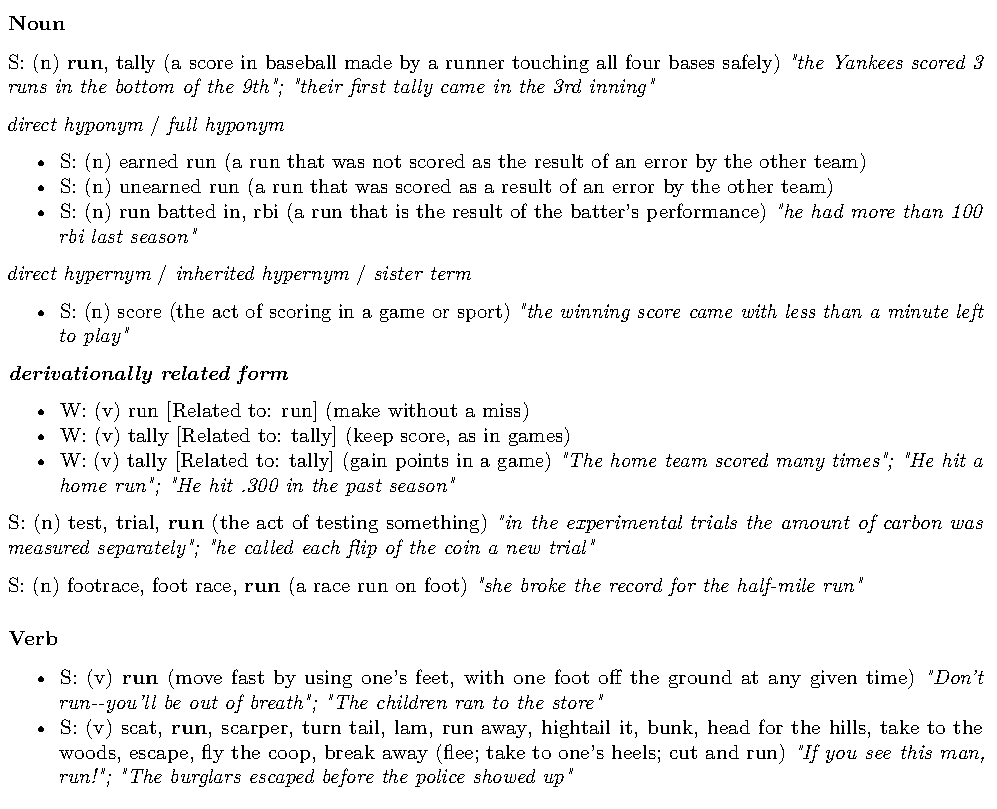
\includegraphics[page=1,width=\textwidth]{Figures/run_wordnet.pdf}}
        }%
        \caption{WordNet result for the query \enquote{run}, truncated for brevity.}\label{fig:example_run}
    \end{center}
\end{figure*}

WordNet lists terms, much like a traditional dictionary, alongside its polysemes but also their homonyms.
Additionally, there is a horizontal association; for any sense, the lemmas that share the row with the target term are synonyms.
This set of synonyms is aptly named \emph{synsets}.
% Furthermore, synset terms can have one or more lexemes, not necessarily singular tokens.
A short description is also provided to clarify the meaning.
These descriptions, hence the meanings for any synset is unique within the WordNet.
During this discussion, we have used sense and synset interchangeably.

WordNet also includes other relationships such as \emph{hypernymy} and \emph{hyponymy}, semantic relation of senses being type-of one another~\cite{miller_nouns_1990}.\footnote{not to be confused with homonymy}
For instance, the term \enquote{building} is a hyponym of \enquote{restaurant} since it encompasses a more general sense; the restaurant is type of a building.
While coffee shop is a hypernym to the restaurant since it is a more specific sense.
% TODO maybe a sense graph here
One other relation is the meronymy, defined as a sense being part of or a member of another~\cite{winston_taxonomy_1987}.
Keeping to our building example, windows are meronym to buildings.
Other relationships exist but listing them is outside the scope of this thesis.
Bottom line is the effort that has gone through to map $117,000$ senses according to different semantic relationships.
% TODO how to typeset numbers?
\textcite{sagot_building_2008} argue that the semantic relationships between senses are not tied to a specific language.
With this assumption at hand, we can infer the effort behind the WordNet does not need to be repeated but can be translated to other languages.

Since it's inception, other projects built lexical databases, using the same WordNet design.
% TODO reference here after chapter 2
\textcite{fellbaum_semantic_1998} talks about the correct terminology that we abide for the thesis; \enquote{As WordNet became synonymous with a particular kind of lexicon design, the proper name shed its capital letters and became a common designator for semantic networks of natural languages}.
Hence \emph{WordNet} refers to English Princeton WordNet, while \emph{wordnets} created for other languages are not stylized.

\section{Multilingual Wordnets}%
\label{sec:multilingual_wordnets}
Authorities list more than 7000\footnote{\url{https://www.ethnologue.com/statistics}} living languages but only 40\footnote{\url{https://w3techs.com/technologies/history_overview/content_language/}} of them have a sizeable presence on the internet.
Among this small fraction, English is the dominant language of the web.
English in not the centrepiece for natural language processing research because of any linguistic attribute.
It is simply the most abundant language on web, giving researchers data to work with.

Natural language processing library spaCy~\footnote{\url{https://spacy.io/}} resorts to lemmatizations such as \emph{=PRON=} to denote pronouns in order to collapse the senses for \enquote{I} \enquote{you}, \enquote{them} etc.\@.
% might be too cheesy
The sense and the accompanying word for being the brother of a person's father or mother differs in Turkish while both collapse in \enquote{uncle} in English.
% \might be too cheesy
Studying other languages can provide insight towards concepts that are not present in English.

Translation, information transfer from foreign languages is a valid way of enriching a language's corpora; if a term that for a sense does not have a match in the target language, it is a good indication for the linguists of that language to look into their lexicons and work towards expanding it~\cite{ibrahim_usta_turkce_2006}.
Further research in the area contributes to languages other than English having access to tools that will incorporate them into the literature.

Open Multilingual WordNet~\cite{bond_survey_2012} set out to discover the effects related to the choice of license for wordnets.
Their criteria for usefulness is the number of citations a publication tied to the wordnet has gotten on literature.
They identified two major problems with the current distributions;
\begin{itemize}
    \item some projects have picked restrictive licenses, effectively barring access to their tools for research purposes.
    \item the structures of the wordnets are not standardized, creating additional cost for creating programs to parse and use the wordnets.
\end{itemize}
In order to overcome the standardization issue, \citeauthor{bond_survey_2012} have aligned the wordnets according to their English Princeton WordNet lemma ids and have written individual scripts to parse them.
They are currently hosting the results from a single source.\footnote{\url{http://compling.hss.ntu.edu.sg/omw/}}

With alignment information at hand, we have created our dataset that we will assume to be perfectly aligned; a golden corpus.
Among the 34 wordnets available on Open Multilingual WordNet, only 6 of them have gloss information available.
Given this thesis will only investigate the ability to map senses using definitions of the sense, we used the subset of Albanian~\cite{ruci_current_2008}, Bulgarian~\cite{simov_constructing_2010}, Greek~\cite{stamou_exploring_2004}, Italian~\cite{pianta_multiwordnet_2002}, Slovenian~\cite{fiser_slownet_2012} and Romanian~\cite{tufis_romanian_2008} wordnets.
Table~\ref{tab:summary_table} shows brief statistics about them.
We should note that the languages of the wordnets used in the thesis are all present in the 40 languages that have a significant presence on the internet that we have mentioned before.
We have constrained this study to use only the freely available wordnets and not considered wordnets that are gated behind restrictive licenses.

\begin{table}[htbp]
    \centering
    \begin{tabular}{llr}
        \toprule%
        \textbf{Name of the Project} & \textbf{Language} & \textbf{Number of Definitions} \\
        \midrule%
        Albanet & Albanian & 4681 \\
        BulTreeBank WordNet & Bulgarian & 4959 \\
        Greek Wordnet & Greek & 18136 \\
        ItalWordnet & Italian & 12688 \\
        Romanian Wordnet & Romanian & 58754 \\
        SloWNet & Slovenian & 3144 \\
        \bottomrule %
    \end{tabular}
    \caption{Summary of the Wordnets used.}\label{tab:summary_table}%
    \label{tab:wordnet_summary}
\end{table}

% \begin{table*}[!hbp]
%     \begin{center}
%         \caption{Summary of the Wordnets used.}\label{tab:summary_table}
%         \begin{tabular}{llrr}
%             \toprule%
%             \textbf{Name of the Project} & \textbf{Language} & \textbf{Number of Definitions} & \textbf{Words Per Definition} \\
%             \midrule%
%             Albanet & Albanian & 4681 & 11.75 \\
%             BulTreeBank WordNet & Bulgarian & 4959 & 12.71 \\
%             % DanNet & Danish    & 784                   & 8.63                           \\
%             Greek Wordnet & Greek & 18136 & 11.24 \\
%             ItalWordnet & Italian & 12688 & 7.33 \\
%             Romanian Wordnet & Romanian & 58754 & 9.98 \\
%             SloWNet & Slovenian & 3144 & 12.68 \\
%             \bottomrule %
%         \end{tabular}
%     \end{center}
% \end{table*}

\section{Thesis Goals}% TODO return here
\label{sec:thesis_goals}
% TODO we assume word embeddings are interchangeable

In this thesis, we will study document matching and document retrieval methods.

We will evaluate existing methods for their performance on cross-lingual document retrieval but our documents are dictionary definitions which are short, descriptive snippets of text.
At the end of this study, we will answer the following research questions;

\begin{enumerate}
    \item Is it possible to create wordnet like lexical databases using unsupervised document matching and retrieval techniques.
    \item How well does the studied techniques perform.
    \item What attributes need to be considered regarding the available data.
\end{enumerate}

\section{Thesis Outline}%
\label{sec:thesis_outline}
\texttt{Fill later\ldots}

% Chapter Template

\chapter{Background Information \& Related Work}%
\label{chap:background_n_related}
% ROUGH DRAFT

James Somers puts down the modern dictionaries by saying \enquote{The definitions are these desiccated little husks of technocratic meaningese, as if a word were no more than its coordinates in semantic space.}~\cite{somers_youre_2014}.
Even though the author criticises the efficient of the dictionary definitions, we will build the thesis on the idea that we can represent senses using their dictionary definitions.

\section{Word Embeddings}%
\label{sec:word_embeddings}

% Surveys used are
% \cite{turney_frequency_2010} -> VSM Survey
% Has the history but omits (rightfully) language modelling stuff (bengio and so on)
% \cite{camacho-collados_word_2018} -> Sense Embeddings Survey (Short section on word embeddings)
% \cite{almeida_word_2019} -> Brasil Survey (Very poorly written, don't want to cite if I can help it)
% \cite{ruder_survey_2017} -> Ruder Survey (Bilingual embeddings, short section on word embeddings)
% http://ruder.io/word-embeddings-1/index.html
% Used as 'what to look for', though some has conflicting information

Recent studies have been using word representations, commonly known as \emph{word embeddings}.
Word embeddings are real valued, dense feature vectors for words.
They are induced in order to map a lexicon to a multidimensional latent space.
This representation allows researchers access to the tools of a broad literature in linear algebra and machine learning.
Since the embeddings and their respective words (labels) can be saved to the disk, researchers have been sharing their models on the internet for other researchers to simply download and use them on their own applications.
Word embeddings acquired this way are often called \emph{pre-trained}.

In this section, we will present a brief history of word embeddings.
At the end of the section, we will study our selected model, \emph{fastText}~\cite{mikolov2018advances}.

Word embeddings is a sprawling subject that has been built upon ideas from probabilistic, statistical and neural network models.
We have omitted approaches that are not used for our study and constrained ourselves only to the literature that lead up to the model we will use. % dilimiz dondugunce

\subsection{History of Word Representations}%
\label{sub:history_of_word_representations}

In order to talk about how words can be mapped to a multidimensional space, first we should talk about how the idea that they can has been theorized.

\subsubsection{Linguistic Background}%
\label{ssub:linguistic_background}

In his \citeyear{harris_distributional_1954} article, \textcite{harris_distributional_1954} introduced his ideas which later came to known as \emph{distributional hypothesis} in the field of linguistics.
He argued that similar words appear within similar contexts.
The famous quote by \textcite{firth_synopsis_1957} captures the idea as;
\enquote{You shall know a word by the company it keeps!}
For instance, the semantic similarity between the terms \emph{jacket} and \emph{coat} can be theoretically proven since they will be accompanied by similar verbs, such as \emph{wear}, \emph{dry clean} or \emph{hang}, and similar adjectives such as \emph{warm} or \emph{leather}.
% is leather an adjective?
However, for a researcher to extract these rules by hand would have been infeasible.

Even though \citeauthor{harris_distributional_1954} argued that \enquote{language is not merely a bag of words}, using unordered collection of word counts to capture the semantic information will be used in the literature and be known as the \emph{bag-of-words} hypothesis.

\subsubsection{Vector Space Model}%
\label{ssub:vector_space_model}

The history of word embeddings is tightly coupled with vector space models.
The vector space models first appeared in the information retrieval field.
Initial vector space model developed by \textcite{salton_vector_1975} and presented in \citetitle{salton_vector_1975}.
It was the first application of bag-of-words hypothesis on a corpus to extract semantic information~\cite{turney_frequency_2010}.
\citeauthor{salton_vector_1975} presented the novel idea of a \emph{document space}, consisting of fixed sized vectors as the columns of a term document matrix.
The dimensions of the vectors were the whole vocabulary of the corpus.

In this space, a document $D_i$ is represented using $t$ distinct terms as a row vector;
\begin{displaymath}
    D_{i} = (d_{i1}, d_{i2}, \ldots, d_{it})
\end{displaymath}
The weights for the index terms are calculated by using the \tfidf{} measure introduced by \textcite{jones_statistical_1972}.
\tfidf{} is the multiplication of two metrics;
\begin{description}
    \item[\emph{tf}] the number of times a term $k$ occurs in a document
    \item[\emph{idf}] the inverse of the number of documents that contain $k$.
\end{description}

\citeauthor{salton_vector_1975} presented their particular weighting scheme where the term frequency is multiplied by the following inverse document frequency for the term $k$.
\begin{displaymath}
IDF_{k} = \ceil[\big]{\log_{2}n} - \ceil[\big]{\log_{2}d_{k}} + 1
\end{displaymath}
% simply log_2(n/d_{k})
Where $n$ is the number of documents in the collection and $d_k$ is the number of documents that consists the term $k$.
The weighting scheme was selected to \enquote{assign the largest weight to those terms which arise with high frequency in individual documents, but are at the same time relatively rare in the collection as a whole}.
Finally, they have cast their similarity function between documents $i$ and $j$, as the inner product between their vectors which corresponds to the cosine similarity.

The vector space model allowed \citeauthor{salton_vector_1975} to handle the similarity between documents as the angle between two vectors.
More importantly, they have shown that there is merit to handling documents as real valued vectors.

\subsubsection{Latent Semantic Analysis}%
\label{ssub:latent_semantic_analysis}

\textcite{deerwester_indexing_1990} introduced latent semantic analysis in order to address a crucial problem with the vector space model.
They have identified that synonyms and homonyms cannot be handled by the naive term document matrix approach due to the fact that vector space model requires the words to match exactly between the two documents.
Synonymity is an issue because the query might have terms that have the same meaning as the target word.
On the other hand, homonyms might match with an unrelated word.
Their model seeks the higher order latent semantic structure in order to learn the \emph{similarity between words}.

Latent semantic analysis starts with a word co-occurrence matrix $X$.
The terms of the matrix is weighted by some weighting scheme.
While original study used raw term frequencies, \tfidf{} is a possibility while \textcite{levy_improving_2015} reports pointwise mutual information (PMI)~\cite{church_word_1990} as a popular choice.
A term document matrix $X$ is then factorized into three matrices using singular value decomposition~\cite{forsythe_computer_1977};
% People don't cite this for some reason, is it wrong?
\begin{displaymath}
    X = T_{0}S_{0}D_{0}'
\end{displaymath}
Where the columns of $T_{0}$ and $D_{0}'$ are orthogonal to each other and $S_{0}$ is the diagonal matrix of singular values.
The singular values of $S_{0}$ can be ordered by size to keep only the $k$ largest elements, setting the others to zero~\cite{deerwester_indexing_1990}.

Their use for the resulting matrix is as follows;
\begin{displayquote}
    Each term or document is then characterized by a vector of weights indicating its strength of association with each of these underlying concepts.
    That is, the \enquote{meaning} of a particular term, query, or document can be expressed by $k$ factor values, or equivalently, by the location of a vector in the $k$-space defined by the factors.
\end{displayquote}
They have used this technique to solve document similarity task and touched upon \emph{word similarity}.
% TODO I can't talk about this paper in a concise way or any way really, return later
% levy_improving_2015 section 2.2 has a very short and nice explanation if you want
Using latent semantic analysis to represent word similarity is later studied by \textcite{landauer_solution_1997}

\subsubsection{Building Upon Distributional Hypothesis}%
\label{ssub:building_upon_distributional_hypothesis}

% \textcite{schutze_dimensions_1992} (intro to information retrieval co-author) is earlier but doesn't appear in any survey, A Survey on Word Representations of Meaning cites later works (Automatic word sense disambiguation), most just skip to lund
% "in order for the dimensions of meaning and the vector representations of words to reflect closeness in meaning faithfully, a global optimization of cooccurrence constraints is necessary, an operation so complex that only a supercomputer can perform it." that's why
% also used a context size of _characters_ because "few long words are better than many short words"
While \citeauthor{deerwester_indexing_1990} studied relatedness between words using vectors, their approach used the whole corpus for the co-occurrence information and the focus was still on the document similarity.

\textcite{schutze_dimensions_1992} proposed \enquote{to represent the semantics of words and contexts in a text as vectors} and built upon word co-occurrence.
They theorized a context window of 1000 characters in order to not consider the whole corpus but only words that are close to the target word to be considered in co-occurrence calculations.
% They used cosine similarity as a measure of semantic relatedness between word vectors.
However, they claimed that the computation power available was not suitable yet to fully tackle the task.

% Lund is not cited as much, is context window important?
% Why did Lund capture associativity instead of semantic relatedness?
% Collobert! This just predicts the next word, not the job of a word in a text
\textcite{lund_producing_1996} took the challenge and experimented upon 160 million words taken from the internet.
They used a context size of 10 words and provided a method to obtain feature vectors to represent the meaning of words.
% maybe talk about the method but seems redundant
However, intricate tuning of word co-occurrence generated associatively similar vectors instead of semantically similar ones.
% Figure 1 of this paper can be adapted here

% Count based approaches to predictive approaches
% Conventional VSM produces high dimensional representations, since the dims. correspond to words in the number can reach millions -> don't know where I got this, can't use it as it probably plagiarism
\subsubsection{Distributed Vector Representations}%
\label{ssub:distributed_vector_representations}
% https://www.gavagai.se/blog/2015/09/30/a-brief-history-of-word-embeddings/
% Wish this post had an author, main takeaways;
% The main difference between these various models (neural language models and distributional semantic models) is the type of contextual information they use.
% LSA and topic models use documents as contexts, which is a legacy from their roots in information retrieval.
% Neural language models and distributional semantic models instead use words as contexts, which is arguably more natural from a linguistic and cognitive perspective.
% These different contextual representations capture different types of semantic similarity; the document-based models capture semantic relatedness (e.g. “boat” – “water”) while the word-based models capture semantic similarity (e.g. “boat” – “ship”).
% This very basic difference is too often misunderstood.

% \textcite{bengio_neural_2000} root word embedding paper.
% EVERYONE says they coined 'word embeddings', doesn't appear in the paper, don't know where people got that
% There is another paper called A Neural Probabilistic Language Model, that came out in 2000
% People pretend that it doesn't exist, we'll use the 2003 one as well, it's just the extended version I think

% So far we've been talking about IR, now this is language models
% For instance Turney Pantel (VSM Survey) doesn't mention bengio or any other word embeddings (2010)

% input layer -> emb. layer -> softmax layer
\textcite{bengio_neural_2003} proposed learning word representations using a feedforward neural network.
Their model would learn feature vectors for words using a predictive approach instead of counting based approaches we have presented until now.
Although neural networks have been proposed to learn a language model~\cite{xu_can_2000}, the main contribution of \citeauthor{bengio_neural_2003} is to use an \emph{embedding layer}, in order to attack \emph{curse of dimensionality}.
For a corpus of $V$ words, there are $|V|$ dimensions for the language model to learn and taking \emph{n-gram} representations into consideration, the problem grows exponentially.
Using $m$ dimensions in the embedding layer allowed \citeauthor{bengio_neural_2003} to represent words using manageable dimensions.
% $|V| >> m$

The setup for the neural network starts with the one hot encoded vector representation of the context for a word $w$.
This context is not a window but similar to statistical models that predicts the word $w$ using the words that lead up to $w$, $w_{}$.
% TODO something about statistical models here
The input layer is projected into an embedding layer, later to a softmax layer to get a probability distribution.
% TODO softmax formula here

However, the softmax layer is computationally expensive to be viable.
% TODO why
Authors reported training times around 3 weeks using 3 to 5 context window sizes and vocabulary sizes around 17000.
% TODO talk about shifting the difficulty elsewhere, instead of full vocabulary dimensions, you just have last layer to worry about

\citeauthor{collobert_unified_2008} suggested a deep neural network model in order to learn feature vectors for various natural language processing tasks.
Their proposed approach for language model is important for our case since it explicitly learned distributed word representations or simply word embeddings.
They have introduced two key ideas;
\begin{itemize}
    \item Instead of using a context window that used words left of the target word to estimate the probability of the target word, they have placed the context window \emph{on} the target window, using $n$ words for left and right of the target word.
    \item They introduced negative examples, where they randomly changed the middle word with a random one. This allowed them to use the ranking cost;
        \begin{displaymath}
            \sum_{s \in S} \sum_{w \in D} \text{max}\big( 0, 1 - f(s) + f(s^w)\big)
        \end{displaymath}
\end{itemize}
\citeauthor{collobert_unified_2008} claim that these additions allowed their system to learn the representation better rather than the probability.

% Turian 2010 doesn't appear much in any of the surveys or word embedding blogs
% but as far as i can tell, they're the first to say word embeddings are useful because they're off the shelf which I want to emphasize
% Like they literally say "With this contribution word embeddings can now be used off-the-shelf as word features, no tuning"

\textcite{p._turian_word_2010} evaluated the performance of different word representations as word features you can include into an existing task.
They summarize their contribution as follows;
\begin{displayquote}
  Word features can be learned in advance in an unsupervised, task-inspecific, and model-agnostic manner.
  These word features, once learned, are easily disseminated with other researchers, and easily integrated into existing supervised NLP systems.
  \textelp{} % TODO want this on it's own line
  With this contribution, word embeddings can now be used off-the-shelf as word features, with no tuning.
\end{displayquote}

% Jointly with \citeauthor{collobert_unified_2008}, \citeauthor{p._turian_word_2010} steered the work on word representations to the today's route.
% They showcased that word embeddings can indeed be used as ready made feature vectors and once trained, can be used for other applications by other researchers.
% Important to note that they reported training times in the order of days, even weeks.

% \textcite{mikolov_distributed_2013} word2vec paper.
% This paper is legendary, talk about skip-gram, hierarchical softmax negative sampling
% If need be, \cite{goldberg_word2vec_2014} -> word2vec explained

word2vec~\footnote{\url{https://github.com/tmikolov/word2vec}} package~\cite{mikolov_distributed_2013,mikolov_linguistic_2013,mikolov_exploiting_2013} popularized the word embeddings.
There are two aspects of the work done by \citeauthor{mikolov_distributed_2013}  that contributed to the fact;
\begin{itemize}
    \item Their model captures the semantic and syntactic attributes of words and phrases on a large scale with good accuracy, trained on billions of words.
    \item Their code and the pre-trained embeddings have been published as open source.
\end{itemize}

by \textcite{mikolov_distributed_2013} brought together the advancements and attractiveness that were brewing in the word embedding research.
First and foremost, they used an efficient loss function for their neural network architecture, the hierarchical softmax. % TODO ref here

With training time under manageable conditions \ldots.
Used negative subsampling, essentially a probability for a word to be discarded by inversely proportional to how frequent it is in the dataset.
Their most famous contribution is the quality of the vectors they have learned.
The theory set out by ? was empirically shown by \citeauthor{mikolov_distributed_2013} by demonstrating that countries and their capital cities exhibited a linear pattern on the PCA.
% TODO simplified graphic here, what is a PCA?

Also element-wise addition in section 5.
% TODO read section 5
They have been hosting their project open source but perhaps more importantly, they published an word2vec pretrained model on English on the internet.
Researchers and industry professionals have been using the embeddings since the semantic similarity between close words were relevant in numerous applications.

% http://blog.aylien.com/overview-word-embeddings-history-word2vec-cbow-glove/
% Ruder says don't dwell on the specific embedding too much
% fasttext is trained on a huge corpus with tuned hyperparameters
% hence the choice of the specific model is not important
\textcite{levy_improving_2015} compared the performance of count based and prediction based word representation models.
Representation algorithms they considered are;
\begin{itemize}
    \item Positive pointwise mutual information (PPMI)~\cite{church_word_1990, bullinaria_extracting_2007}
    \item Singular Value Decomposition on PPMI Matrix (Latent Semantic Analysis)~\cite{deerwester_indexing_1990}
    \item Skip-Gram with Negative Sampling~\cite{mikolov_distributed_2013}
    \item Global Vectors for Word Representation~\cite{pennington_glove_2014}
\end{itemize}
They found out that choice of a particular algorithm played an insignificant role compared to choosing the right \emph{hyperparameters}.
They used this finding to counter the results reported by \textcite{baroni_dont_2014} which claimed that predictive models outperformed count based models.
On the other hand, \citeauthor{levy_improving_2015} noted that \citeauthor{baroni_dont_2014} used count based models without hyperparameter tuning, denying them from \enquote{tricks} developed in the word representation literature.

\subsubsection{fastText}%
\label{ssub:fasttext}

%Finally, word2vec lead up to \textcite{bajo}
% bag of character n-grams, no need to worry about mophological structure of the language, can induce oov words if parts of it are available,
% Ruder survey demonstrated how good at compositing they are *citation needed*
Armed with the fact that a good word representation model should have tuned hyperparameters and should be trained on a large dataset, we set our sights on \emph{fastText}~\footnote{\url{https://fasttext.cc/}}.
From their website, fastText is (a) \enquote{Library for efficient text classification and representation learning}.
Ideas behind it are presented in \textcite{mikolov2018advance}.
Overall, it builds upon word2vec~\cite{mikolov_distributed_2013} by adding position dependent features presented in \textcite{mnih_learning_2013} and character n-grams suggested on \textcite{bojanowski_enriching_2016}.
On their website, they are currently hosting pre-trained word embeddings for 157 languages, built from \emph{Common Crawl} and \emph{Wikipedia} data.

\section{Bilingual Word Embeddings}%
\label{sec:bilingual_word_embeddings}

Cross lingual embedding models optimize similar objectives.
Only source of variation is due to the data used and the monolingual regularization objectives employed~\cite{ruder_survey_2017}.

\section{Document Retrieval}%
\label{sec:document_retrieval}

\section{Approaches in Wordnet Generation}%
\label{sec:approaches_in_wordnet_generation}

% from Leveraging Parallel Corpora and Existing Wordnets for Automatic Construction of the Slovene Wordnet
WordNet generation is broken down into 4 categories
\begin{enumerate}
    \item Expand model, \textcite{vossen_introduction_1998}, fixed synsets are translated from English to target language.
    \item Link English entries from machine-readable bilingual dictionaries to English Princeton WordNet senses~\textcite{knight_building_1994}.
    \item Taxonomy parsing~\textcite{farreres_using_1998}.
    \item Ontology matching~\textcite{farreres_towards_2004}
\end{enumerate}

\textcite{sagot_building_2008} built a French wordnet.

\textcite{gordeev_unsupervised_2018} uses unsupervised cross-lingual embeddings to match cross-lingual product classifications.
Working on taxonomy matching, they use out of domain pre-trained embeddings due to small size of their corpora and investigate methods using untranslated and translated text.

\textcite{lesk_automatic_1986} represent words using their gloss.
Relied upon traditional dictionaries.
\textcite{banerjee_adapted_2002} developed on lesk algorithm and included WordNet definitions.
\textcite{khodak_automated_2017} used word embeddings and WordNet.

\textcite{metzler_similarity_2007} talked about short text retrieval and lexical matching.
They reported that lexical matching is good for finding semantically identical matches.

\textcite{xiao_distributed_2014} another embedding paper.

\textcite{kusner_word_2015} is Word Mover's Distance.

\textcite{balikas_cross-lingual_2018} suggested using optimal transport for cross-lingual document retrieval.

\textcite{arora_simple_2016} simple but tough-to-beat baseline for sentence embeddings.

\textcite{klementiev_inducing_2012} base paper for cross lingual word embeddings?

% Chapter Template
\chapter{Unsupervised Matching}%
\label{chap:unsupervised_matching}

%%% ROUGH FIRST DRAFT

\section{Linear Assignment Using Sentence Embeddings}%
\label{sec:linear_assignment_using_sentence_embeddings}
% TODO down below two tracks for sentence embeddings will crash, print out and clean up
From word embeddings that represented single tokens, research also tackled the representation of longer pieces of text like documents, paragraphs and sentences.
Implementations like \textcite{le_distributed_2014} extended the skip-gram idea of \textcite{mikolov_distributed_2013} to represent \emph{paragrahs} as feature vectors and used them to predict surrounding paragraphs in the text.
While approaches like \textcite{kiros_skip-thought_2015} trained an encoder that constructed surrounding sentences to learn to learn sentence representations.
% TODO This can go to chapter2 and get expanded if need be
However, there is an assumption of a continuous text for the given models.
When the text that we would like to show on a latent space is not part of a longer piece of text but \emph{discrete} pieces, that assumption does not hold.
With the dictionary definitions, we have such a case.
Our dictionary definitions are comprised of 10 to 11 words and there is no relation from one distinct dictionary definition to another.
% TODO reference the wordnet statistics table when you decide on where to put it
In other words, they are not continuous.
One other case where a similar situation occurs is \emph{twitter}.
\emph{Tweets} are short pieces of text due to the 280 character constraint imposed by the platform.
With such short pieces of text, instead of paragraph embeddings, we can talk about \emph{sentence embeddings}.
A sentence embedding model should ideally capture the collective meaning of the short text where every word is potentially informative.

Thankfully, \textcite{wieting_towards_2015} studied sentence embeddings and reported that averaging word embeddings that make up a sentence to get sentence embeddings is a valid and surprisingly effective approach.
\textcite{arora_simple_2016} built upon that idea and presented that weighed average of word vectors perform so well, they decided to call it; \citetitle{arora_simple_2016}.
In the suggested approach, word embeddings are weighed with a scale called \emph{smooth inverse frequency}.
Smooth inverse frequency is reported as $a/(a + p(w))$ where $a$ is a parameter and $p(w)$ is the word frequency.
The authors point out that the metric is similar to \tfidf{} weighting scheme if \enquote{one treats a \enquote{sentence} as a \enquote{document} and make the reasonable assumption that the sentence doesn't typically contain repeated words}.
These assumptions hold for us so we scaled our word embeddings using \tfidf{} weights to get sentence embeddings.

Parallel to
\textcite{zhao_ecnu_2015} used two approaches for SemEval-2015 Task 2: Semantic Textual Similarity~\footnote{\url{http://alt.qcri.org/semeval2015/task2/}}.
First, for a sentence $S = (w_{1}, w_{2}, \dots, w_{s})$ where the length of the presumably small sentence is $|S| = s$ and the word embedding of a $w_t$ is $v_t$;
\begin{itemize}
    \item They summed up the word embeddings of the sentence $\sum_{t \in S}v_{t}$
    \item Used information content~\cite{saric_takelab_2012} to weigh each word's LSA vector $\sum_{t \in S} I(w_t) v_{t}$
\end{itemize}
Both approaches results in a vector that is in the same dimensions $R^{d}$ as the original word representations.

\textcite{edilson_a._correa_nilc-usp_2017} expanded upon this simple yet effective idea to tackle the SemEval-2017 Task 4\footnote{\url{http://alt.qcri.org/semeval2017/task4}}, Sentiment Analysis in Twitter.
In order to acquire embeddings that represented \emph{tweets}, they weighed the word embeddings that made up a tweet; $\text{tweet}_i = (w_{i1}, w_{i2}, \dots, w_{im})$ with the \tfidf{} weights.
For the \tfidf{} calculation, they cast individual weights as documents so that term frequency become the term count in a single tweet while document frequency become the number of tweets the term $w_t$ occurs.

We have mentioned that our dictionary definitions are not continuous.
Yet, we advocate using \tfidf{} weights to weigh our word embeddings to get sentence embeddings.
In order to clarify, let us present Table~\ref{tab:en_it_examples}.
\begin{table}
    \centering
    \caption{Some definitions from English Princeton WordNet}%
    \label{tab:en_it_examples}
    \begin{tabular}{l}
        \toprule
        turn red, as if in embarrassment or shame \\
        a feeling of extreme joy \\
        a person who charms others (usually by personal attractiveness) \\
        so as to appear worn and threadbare or dilapidated \\
        a large indefinite number \\
        distributed in portions (often equal) on the basis of a plan or purpose \\
        a lengthy rebuke \\
        \bottomrule
    \end{tabular}
\end{table}

% For sentence embeddings, first a \tfidf{} matrix is constructed.
For the \tfidf{} calculations, we followed a similar approach.
The term frequency is the raw count of a term in a dictionary definition.
While the document frequency is the number of dictionary definitions where $w_t$ occurs.

Then, with the term-embedding matrix at hand, we have calculated definition embeddings using;
\begin{equation}
    S_{\text{emb}}(S) = \sum_{w_{i} \in S} \varB{tf_{w_{i},S}-idf_{w_i}} \cdot Emb_{w}(w_{i})
\end{equation}
Every word that makes up a definition is scaled by its vector in ${\rm I\!R}^n$, then concatenated to form sentence embeddings on ${\rm I\!R}^n$.
% TODO cost matrix
% Bipartite graph or matrix
% Give the assumption, defintions are one-to-one
Given the N vectors from source and target language, we hypothesize that there exists a matching where every source definition vector is perfectly mapped to one target vector.
Given that this problem naively iterates over $N!$ matchings, we have looked into an algorithm.

%%% TODO lapjv %%%
% https://blog.sourced.tech/post/lapjv/
%
\section{Linear Assignment Algorithm}%
\label{sec:linear_assignment_algorithm}
% Ok jonker volgenant is super complicated
% can I just say I'm using linear assignment? maybe talk about hungarian algortihm a bit



\section{Results}%
\label{sec:results}

\begin{table}[htbp]
    \centering
    \begin{tabular}{lrrr}
        \toprule
& \multicolumn{3}{c}{Percentage of Correctly Matched Definitions} \\
\cmidrule(lr){2-4}
        \textbf{Language} & \textbf{fastText 1M} & \textbf{fastText 500k} & \textbf{Numberbatch} \\
        \midrule
        bg & 0.39 & 0.41 & 0.19 \\
        el & 0.37 & 0.38 & 0.14 \\
        it & 0.28 & 0.28 & 0.36 \\
        ro & 0.39 & 0.39 & 0.20 \\
        sl & 0.15 & 0.15 & 0.06 \\
        sq & 0.55 & 0.54 & 0.27 \\
        \bottomrule
    \end{tabular}
    \caption{Linear Assignment Using 2000 Definitions}%
    \label{tab:lapjv_2000}
\end{table}

\begin{table}[htbp]
    \centering
    \begin{tabular}{lrrr}
        \toprule
& \multicolumn{3}{c}{Percentage of Correctly Matched Definitions} \\
\cmidrule(lr){2-4}
        \textbf{Language} & \textbf{fastText 1M} & \textbf{fastText 500k} & \textbf{Numberbatch} \\
        bg & 0.35 & 0.36 & 0.18 \\
        el & 0.36 & 0.36 & 0.12 \\
        it & 0.25 & 0.25 & 0.32 \\
        ro & 0.36 & 0.37 & 0.19 \\
        sl & 0.11 & 0.11 & 0.05 \\
        sq & 0.39 & 0.40 & 0.19 \\
        \bottomrule
    \end{tabular}
    \caption{Linear Assignment Using 3000 Definitions}%
    \label{tab:lapjv_3000}
\end{table}

\begin{table}[htbp]
    \centering
    \begin{tabular}{lrrr}
        \toprule
& \textbf{fastText 1M} & \textbf{fastText 500k} & \textbf{Numberbatch} \\
\midrule
        Best & 0.55 & 0.54 & 0.36 \\
        Worst & 0.11 & 0.11 & 0.05 \\
        Average & 0.33 & 0.33 & 0.19 \\
        \bottomrule
    \end{tabular}
    \caption{Summary of Linear Assignment}%
    \label{tab:lapjv_summary}
\end{table}

% Chapter Template

\chapter{Unsupervised Retrieval}%
\label{chap:unsupervised_retrieval}

\section{Cross Lingual Document Retrival}%
\label{sec:cross_lingual_document_retrival}

\subsection{Optimal Transport}%
\label{sub:optimal_transport}

\subsection{Sinkhorn}%
\label{sub:sinkhorn}







% Chapter Template

\chapter{Supervised Validation}%
\label{chap:supervised_validation}

The approaches we have presented so far work fully unsupervised.
Given two collections of definitions, we have tried to retrieve the definition(s) that represented the same meaning.
However, given the moderately sized data in our hands we have accepted as \enquote{golden}, we studied the feasibility of training an encoder~\cite{sutskever_sequence_2014}, where the objective is to learn whether the pair of definitions entail the same sense across languages.

Recurrent Neural Network (RNN) architectures improve upon the prototypical neural network model by introducing a \emph{memory} for the connections in the network~\cite{rumelhart_learning_1986}.
By updating the hidden unit over time using the output of the previous time step, the model can \emph{remember} features of the input signal for later inputs.
% TODO figure here
%RNN seemed fitting for our case given their success on tasks that require a model to \emph{remember} previous signals over a long sequence of inputs\cite{gers_lstm_2001,jean_using_2014}.
One particular architecture of RNNs propsed by \textcite{hochreiter_long_1997} is \emph{long short-term memory} (LSTM).
LSTM models have been successful on language modelling tasks~\cite{sutskever_sequence_2014}, handwriting recognition~\cite{graves_unconstrained_2008,graves_novel_2009} and machine translation with a focus on rare words~\cite{luong_addressing_2014} to name a few.
Highlight of these results are that LSTM has an advantage on tasks that require contextual information to persist over long periods of time~\cite{graves_long_2012}.
Furthermore, LSTMs do not require fixed input vectors, which is a necessity for us since our definition pairs do not have to be the same size.

\subsection{Vanishing Gradient Problem}%
\label{sub:vanishing_gradient_problem}

LSTM is borne out of the need to address the \emph{vanishing gradient problem}~\cite{hochreiter_long_1997, bengio_learning_1994}.
On the original publication by \textcite{hochreiter_long_1997}, a crucial shortcoming of RNNs have been identified as their slow rate of training which may not converge in the end at all.
Independently, \textcite{bengio_learning_1994} suggested that the problem stems from the choice between the conservation of the previous inputs versus resisting against the noise they accumulate.
Figure~\ref{fig:vanishing_gradients}, adapted from \textcite{graves_long_2012} illustrates the problem using shades as the influence of input over neural network units.

\begin{figure}[htbp]
    \centering
    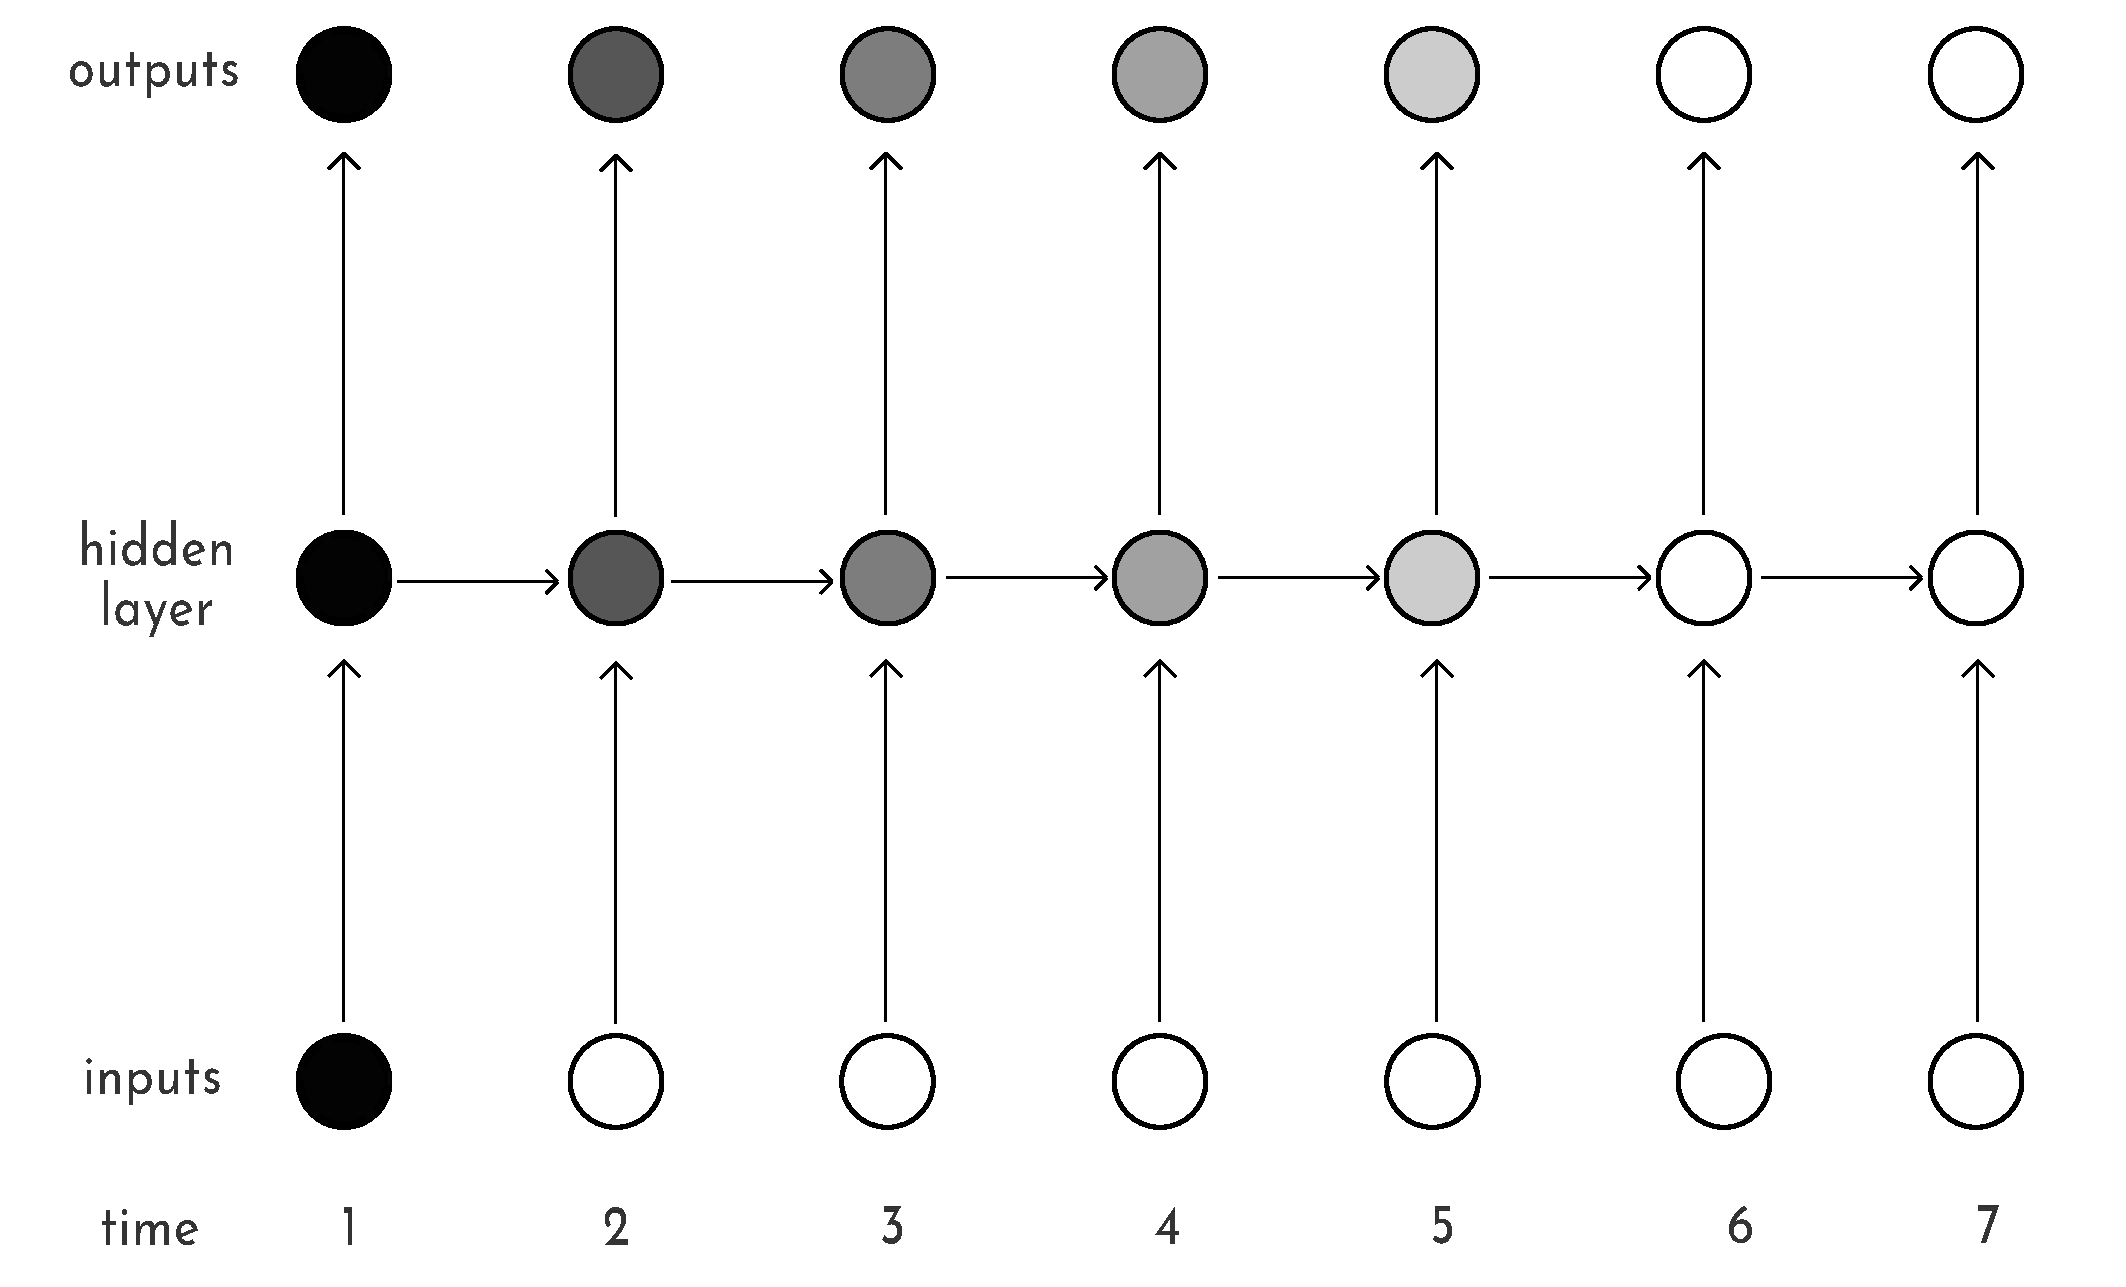
\includegraphics[page=1,width=\textwidth]{Figures/outputs_hiddenlayer.pdf}
    \caption{Graphical representation of vanishing gradient problem where the shades of the nodes represent the influence of the input signal, adapted from Figure 4.1 of \textcite{graves_long_2012}}%
    \label{fig:vanishing_gradients}
\end{figure}

% Input -> will cell learn/change
% Forget -> will cell reset
% Output -> Will cell propagate

%The issue is related to a natural disadvantage of Recurrent Neural Networks (RNN).
As the input signal traverses the units of an RNN, it either diminishes or blows up~\cite{graves_long_2012}.
A long line of solutions were proposed such as decomposing structures so that only unexpected ones can be relevant.
% TODO give more solutions here

\subsection{Long Short-Term Memory}%
\label{sub:lstm}

LSTM is the solution highlighted by \textcite{graves_long_2012} as a recurrent neural network model that can work over temporally distant input signals while preserving their influence or diminishing their noise.
The centrepiece idea is to use a \emph{constant error carousel}, special cells that enforce a constant error flow.
In the original paper, this complex unit is named \emph{memory cell}~\cite{hochreiter_long_1997}.
Using an \emph{input gate}, the cell is updated if the current input is relevant and using an \emph{output gate}, the unit will not update other cells if the current input is not relevant.
A simplified overview of the suggested model is presented in Figure~\ref{fig:simple_lstm}.

\begin{figure}[htbp]
    \centering
    \incfig{simple_lstm}
    \caption{Simplified long short-term memory cell architecture}%
    \label{fig:simple_lstm}
\end{figure}
% We kept forward pass and backprop equations out because no time and out of scope hopefully

Multiple arrows denote input from current time frame and recurrent connections.
$\odot$ symbol denotes multiplication.
By weighing the input and output gates between 0 and 1, the impact of the current input can be adjusted.
Overall, input gate controls how much cell will learn and output gate controls how much the cell will propagate.
Figure~\ref{fig:lstm_preserves} adapted from \textcite{graves_long_2012} illustrates how the LSTMs operate against vanishing gradient.

\begin{figure}[htbp]
    \centering
    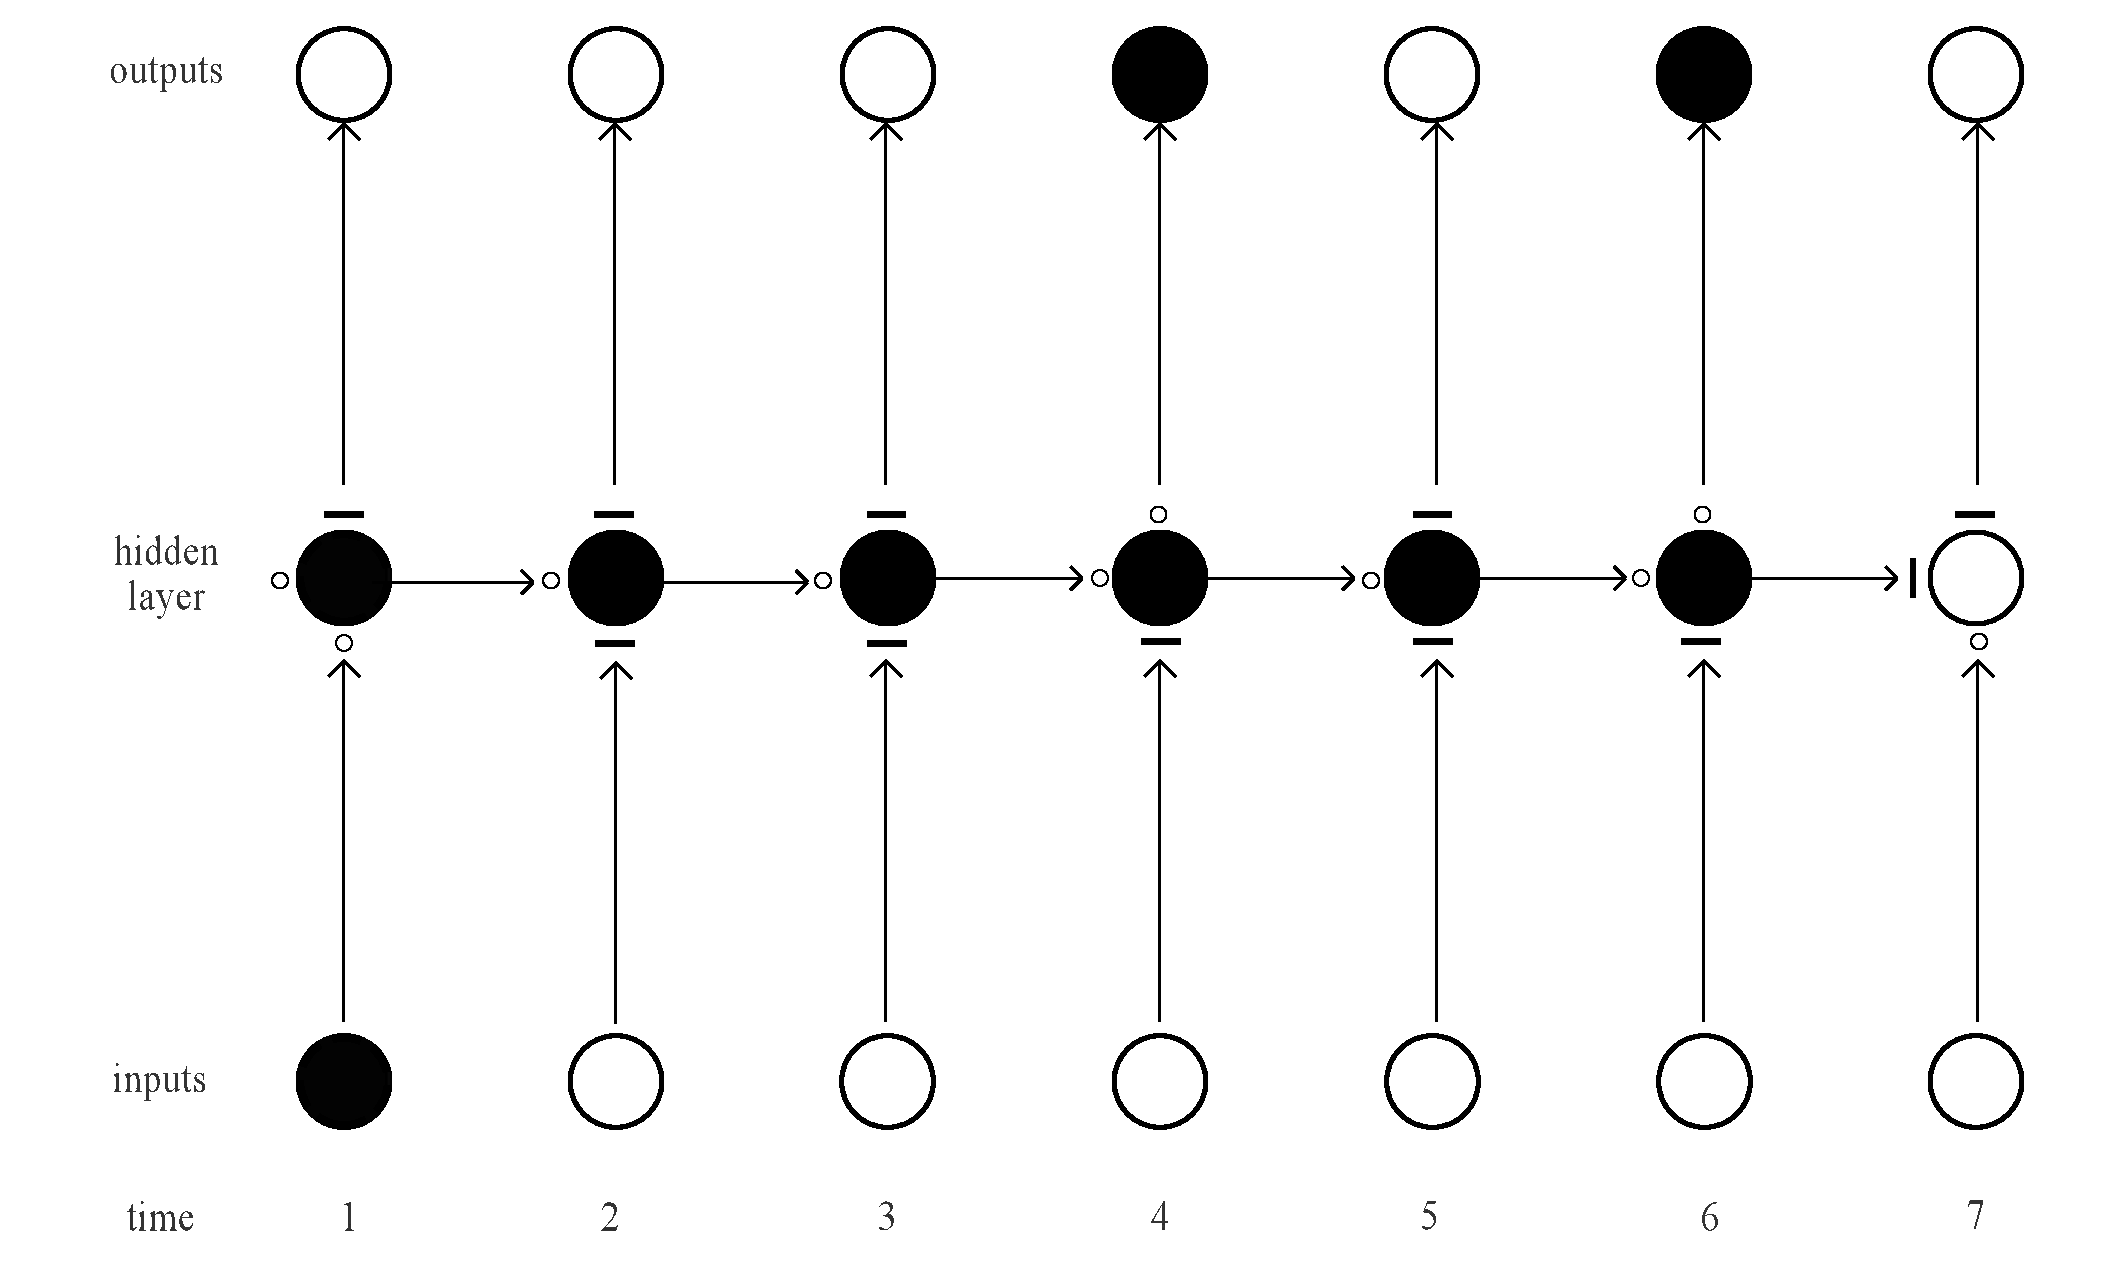
\includegraphics[page=1,width=\textwidth]{Figures/outputs_hiddenlayer2.pdf}
    \caption{Preserving the input signal through blocking (-) or allowing (O) the input signal, adapted from Figure 4.4 of \textcite{graves_long_2012}}%
    \label{fig:lstm_preserves}
\end{figure}

% forget gate
Two gates on top of the cell structure model got extended with a third \emph{forget gate} by \textcite{gers_learning_2000}.
The aim was to handle input sequences that are not segmented in a predictable manner.
The proposed forget gate is implemented to \emph{reset} the cell.
When a cell state got irrelevant due to a change in problem domain, forget gate gradually resets the cell state instead of erroneous activations from the input gate.

% peephole connections
Another extension came in the form of \emph{peephole connections} by \textcite{gers_learning_2003}.
By allowing internal gates to inspect the cell state, they have shown improvements on non-linear tasks.

% \textcite{pascanu_difficulty_2012}

The finalized model with input, forget and output gates as well as the internal peephole connections was debuted in \textcite{graves_framewise_2005}.
In their expansive study comparing 8 LSTM variants over 15 years of CPU time, \textcite{greff_lstm_2017} named this model the \enquote{vanilla LSTM}.
This particular form of LSTM is commonly used~\cite{sutskever_sequence_2014}.
The real valued vectors are denoted alongside their update time step ${(\cdot)}_t$ such that $t \in {1, \dots, T}$.
Updates are performed on the input gate $i_t$, memory cell $c_t$, forget gate $f_t$ and output gate $o_t$.
We show the updates over weight matrices $W_i, W_f, W_c$ and $W_o$ via the use of recurrent weights $R_i, R_f, R_c$ and $R_o$ and bias vectors $b_i, b_f, b_c$ and $b_o$.
Peephole connections are shown using $p_{\cdot}$ for input, forget and output gates as $p_{i}, p_{f}$ and $p_{o}$ respectively.
Finally, the input is a sequence of data in the form of $(x_1, x_2, \dots, x_T)$ and the model outputs real valued vector $y_{t}$ at the time step $t$.

\begin{equation}
    i^{t} = \sigma\left(W_{i}x^{t} + R_{i}y^{t-1} + p_{i} \odot c^{t-1} + b_{i}\right)
\end{equation}

\begin{equation}
    f^{t} = \sigma\left(W_{f}x^{t} + R_{f}y^{t-1} + p_{f} \odot c^{t-1} + b_{f}\right)
\end{equation}

\begin{equation}
    \bar{c^{t}} = W_{c}x^{t} + R_{c}y^{t-1} + b_{c}
\end{equation}

\begin{equation}
    c_{t} = \tanh\left(i^{t} \odot \bar{c^{t}} + f_{t} \odot c^{t-1}\right)
\end{equation}

\begin{equation}
    o^{t} = \sigma\left(W_{o}x^{t} + R_{o}y^{t-1} + p_{o} \odot c^{t} + b_{o}\right)
\end{equation}

\begin{equation}
    y^{t} = \tanh(o_{t}) \odot c^{t}
\end{equation}

Where $\sigma(\cdot)$ is the \emph{logistic sigmoid} function $\sigma(x) = \frac{1}{1 + e^{-x}}$ and pointwise vector multiplication is denoted using $\odot$.
The recurrence holds via the usage of signals from the previous time steps $(\cdot)^{t-1}$.

\subsection{Siamese Long Short-Term Memory}%
\label{sub:siamese_long_short_term_memory}

Recently, \textcite{mueller_siamese_2016} proposed a \emph{siamese} model to solve sentence similarity problem.
They suggest using two networks and denote them as LSTM$_a$ and LSTM$_b$.
The weights are shared between the networks such that LSTM$_a = $ LSTM$_b$.
The Manhattan distance is used as the measure of similarity between

We extend the siamese network architecture by using bilingual word embeddings.


% Optimizer adelta
\textcite{zeiler_adadelta_2012}

% Mean squared error loss

% https://keras.io/layers/recurrent/ implementation details here

% Chapter Template

\chapter{Experiments and Evaluation}%
\label{chap:experiments_and_evaluation}

We experimented with in domain \emph{fasttext} embeddings.
We have trained Romanian and Bulgarian embeddings and ran the WMD and Sinkhorn experiments.
The performance dropped to the quarter of pre-trained embeddings so we have not repeated the experiments for other language corpora.

We have evaluated our embeddings using the standard bilingual lexicon extraction as a general measure for their performance.
Although \textcite{ruder_survey_2017} and \textcite{glavas_how_2019} both say you should evaluate them using downstream tasks.

\begin{table}[htbp]
    \centering
    \begin{tabular}{lrrr}
        \toprule
        \textbf{Language} & \textbf{FastText 1M} & \textbf{FastText 500k} & \textbf{numberbatch} \\
        \midrule
        bg & 33.61 & 35.17 & 51.97 \\
        el & 37.37 & 39.58 & 30.35 \\
        it & 58.20 & 59.28 & 50.37 \\
        ro & 37.33 & 38.71 & 64.17 \\
        sl & 21.42 & 22.91 & 74.74 \\
        sq & 24.46 & 25.36 & 58.63 \\
        \bottomrule
    \end{tabular}
    \caption{Accuracy Scores of the Vectors Aligned Using VecMap}%
    \label{tab:accuracy_results}
\end{table}

\begin{table}[htbp]
    \centering
    \begin{tabular}{lrrr}
        \toprule
        \textbf{Language} & \textbf{FastText 1M} & \textbf{FastText 500k} & \textbf{numberbatch} \\
        \midrule
        bg & 96.43 & 93.36 & 17.53 \\
        el & 94.44 & 90.28 & 12.15 \\
        it & 97.93 & 95.97 & 41.08 \\
        ro & 97.06 & 94.91 & 16.4 \\
        sl & 94.67 & 90.73 & 9.23 \\
        sq & 83.59 & 80.92 & 9.51 \\
        \bottomrule
    \end{tabular}
    \caption{Coverage Scores for the Vectors Aligned Using VecMap}%
    \label{tab:coverage_results}
\end{table}

% Chapter Template

\chapter{Chapter Title Here} % Main chapter title

\label{Chapter7} % Change X to a consecutive number; for referencing this chapter elsewhere, use \ref{ChapterX}

%----------------------------------------------------------------------------------------
%	SECTION 1
%----------------------------------------------------------------------------------------

\section{Main Section 1}

Lorem ipsum dolor sit amet, consectetur adipiscing elit. Aliquam ultricies lacinia euismod. Nam tempus risus in dolor rhoncus in interdum enim tincidunt. Donec vel nunc neque. In condimentum ullamcorper quam non consequat. Fusce sagittis tempor feugiat. Fusce magna erat, molestie eu convallis ut, tempus sed arcu. Quisque molestie, ante a tincidunt ullamcorper, sapien enim dignissim lacus, in semper nibh erat lobortis purus. Integer dapibus ligula ac risus convallis pellentesque.

%-----------------------------------
%	SUBSECTION 1
%-----------------------------------
\subsection{Subsection 1}

Nunc posuere quam at lectus tristique eu ultrices augue venenatis. Vestibulum ante ipsum primis in faucibus orci luctus et ultrices posuere cubilia Curae; Aliquam erat volutpat. Vivamus sodales tortor eget quam adipiscing in vulputate ante ullamcorper. Sed eros ante, lacinia et sollicitudin et, aliquam sit amet augue. In hac habitasse platea dictumst.

%-----------------------------------
%	SUBSECTION 2
%-----------------------------------

\subsection{Subsection 2}
Morbi rutrum odio eget arcu adipiscing sodales. Aenean et purus a est pulvinar pellentesque. Cras in elit neque, quis varius elit. Phasellus fringilla, nibh eu tempus venenatis, dolor elit posuere quam, quis adipiscing urna leo nec orci. Sed nec nulla auctor odio aliquet consequat. Ut nec nulla in ante ullamcorper aliquam at sed dolor. Phasellus fermentum magna in augue gravida cursus. Cras sed pretium lorem. Pellentesque eget ornare odio. Proin accumsan, massa viverra cursus pharetra, ipsum nisi lobortis velit, a malesuada dolor lorem eu neque.

%----------------------------------------------------------------------------------------
%	SECTION 2
%----------------------------------------------------------------------------------------

\section{Main Section 2}

Sed ullamcorper quam eu nisl interdum at interdum enim egestas. Aliquam placerat justo sed lectus lobortis ut porta nisl porttitor. Vestibulum mi dolor, lacinia molestie gravida at, tempus vitae ligula. Donec eget quam sapien, in viverra eros. Donec pellentesque justo a massa fringilla non vestibulum metus vestibulum. Vestibulum in orci quis felis tempor lacinia. Vivamus ornare ultrices facilisis. Ut hendrerit volutpat vulputate. Morbi condimentum venenatis augue, id porta ipsum vulputate in. Curabitur luctus tempus justo. Vestibulum risus lectus, adipiscing nec condimentum quis, condimentum nec nisl. Aliquam dictum sagittis velit sed iaculis. Morbi tristique augue sit amet nulla pulvinar id facilisis ligula mollis. Nam elit libero, tincidunt ut aliquam at, molestie in quam. Aenean rhoncus vehicula hendrerit.


%----------------------------------------------------------------------------------------
%	THESIS CONTENT - APPENDICES
%----------------------------------------------------------------------------------------

\appendix % Cue to tell LaTeX that the following "chapters" are Appendices

% Include the appendices of the thesis as separate files from the Appendices folder
% Uncomment the lines as you write the Appendices

\chapter{Case Study - Aligning a Turkish Dictionary and English Princeton WordNet}%
\label{app:case_study}
\begin{longtable}{p{.50\textwidth} p{.50\textwidth}}
    \toprule
    \textbf{Turkish Definition} & \textbf{English WordNet Definition} \\
    \midrule
    \endfirsthead
    \multicolumn{2}{c}%
    {\tablename\ \thetable\ -- \textit{Continued from previous page}} \\
    \midrule
    \textbf{Turkish Definition} & \textbf{English WordNet Definition} \\
    \midrule
    \endhead
    \multicolumn{2}{r}{\textit{Continued on next page}} \\
    \endfoot
    \midrule
    \endlastfoot
    birdenbire duyulan ağrı ya da türlü heyecanları anlatır & an absence of emotion or enthusiasm \\
    \cmidrule(rl){1-2}
    meyve bisküvi vb ile yapılan bir i̇ngiliz tatlısı & a small hard fruit \\
    \cmidrule(rl){1-2}
    yalıtım tecrit & a thin coating or layer \\
    \cmidrule(rl){1-2}
    bulgu araz & a pattern of symptoms indicative of some disease \\
    \cmidrule(rl){1-2}
    42195 m’lik en uzun yaya koşusu uzunkoşu & any long ditch cut in the ground \\
    \cmidrule(rl){1-2}
    benzer olma durumu müşabehet & the quality of being similar \\
    \cmidrule(rl){1-2}
    var olan bulunan & something that is lost \\
    \cmidrule(rl){1-2}
    parmakların kapanmasıyla elin aldığı biçim & handwear covers the hand and wrist \\
    \cmidrule(rl){1-2}
    zayıf olma durumu & any strong feeling \\
    \cmidrule(rl){1-2}
    bir süreç içindeki durumlardan her biri basamak aşama rütbe mertebe & the effect of one thing or person on another \\
    \cmidrule(rl){1-2}
    bir birimin bölündüğü eşit parçalardan birini ya da birkaçını anlatan sayı & a unit of spoken language larger than a phoneme \\
    \cmidrule(rl){1-2}
    haşhaş sütünü toplamakta kullanılan kaşık & grass mowed and cured for use as fodder \\
    \cmidrule(rl){1-2}
    bir şeyi yapmayı önceden isteyip düşünme maksat & an act of intending a volition that you intend to carry out \\
    \cmidrule(rl){1-2}
    i̇pekböceği kozaları çözülerek çıkarılan ve dokumacılıkta kullanılan çok ince esnek ve parlak tel & a very strong thick rope made of twisted hemp or steel wire \\
    \cmidrule(rl){1-2}
    anadolu’nun doğu ve kuzey bölgelerinde en çok erzurum yöresinde el ele tutuşarak oynanan bir oyun & game a players turn to take some action permitted by the rules of the game \\
    \cmidrule(rl){1-2}
    başkalarından saklanan duyurulmayan saklı kalan mahrem & a consecrated place where sacred objects are kept \\
    \cmidrule(rl){1-2}
    bir kimseye ya da bir şeye karşı belli tavır takınmak & a feeling of sympathy for someone or something \\
    \cmidrule(rl){1-2}
    tarihsel gelişme içinde belirli bir üretim ilişkisinin belirli bir aşamasında bir arada yaşayan insanların tümü & a large number of things or people considered together \\
    \cmidrule(rl){1-2}
    bir cismin herhangi bir yöndeki uzanımı & a relatively small granular particle of a substance \\
    \cmidrule(rl){1-2}
    organizmada birtakım değişikliklerin ortaya çıkmasıyla fizyoloji görevlerinin bozulması durumu sayrılık maraz esenlik” karşıtı & an impairment of health or a condition of abnormal functioning \\
    \cmidrule(rl){1-2}
    yolcu ve gezmenlere geceleme olanağı sağlamak bunun yanında yemek eğlence gibi  türlü hizmetleri sunmak ereğiyle kurulmuş işletme & a building where travelers can pay for lodging and meals and other services \\
    \cmidrule(rl){1-2}
    hükümdar ailesinden olan erkeklere verilen san & female of any member of the dog family \\
    \cmidrule(rl){1-2}
    orduda yazı işleri ile uğraşan er ya da erbaş & a verbal or written request for assistance or employment or admission to a school \\
    \cmidrule(rl){1-2}
    düşmanın gelmesi beklenen yollar üzerinde askeri önem taşıyan kentlerde geçit ve darboğazlarda güvenliği sağlamak için yapılan kalın duvarlı  burçlu mazgallı yapı & an area within a building enclosed by walls and floor and ceiling \\
    \cmidrule(rl){1-2}
    i̇çi su ya da hava dolu ufak kabartı ya da kürecik & water in small drops in the atmosphere blown from waves or thrown up by a waterfall \\
    \cmidrule(rl){1-2}
    hava ya da herhangi bir akışkanı bir yerden başka bir yere basınç yoluyla aktarmaya yarayan makine & a vertical flue that provides a path through which smoke from a fire is carried away through the wall or roof of a building \\
    \cmidrule(rl){1-2}
    başkalarınca bilinmesi sakıncalı görülen bir gerçeği saklamaktan vazgeçip açıklama söyleme bildirme & an acknowledgment of the truth of something \\
    \cmidrule(rl){1-2}
    bir bilim sanat meslek dalıyla ya da bir konu ile ilgili özel ve belirli bir kavramı olan sözcük ıstılah & an occupation requiring special education especially in the liberal arts or sciences \\
    \cmidrule(rl){1-2}
    bir kilidi açıp kapamak için kullanılan araç açar açkı & a fastener fitted to a door or drawer to keep it firmly closed \\
    \cmidrule(rl){1-2}
    i̇şletilmek için bir yere ödünç verilen paraya karşılık alınan kâr ürem işlenti nema & a fixed charge for borrowing money usually a percentage of the amount borrowed \\
    \cmidrule(rl){1-2}
    yeryüzü parçası yerey yer toprak alan & sloping land especially the slope beside a body of water \\
    \cmidrule(rl){1-2}
    yiyecek koymaya yarar az derin ve yayvan kap & metal or earthenware cooking vessel that is usually round and deep often has a handle and lid \\
    \cmidrule(rl){1-2}
    yerleşik toplumsal düzeni köklü hızlı ve geniş kapsamlı olarak niteliksel değiştirme ve yeniden biçimlendirme eylemi inkılap & an extended social group having a distinctive cultural and economic organization \\
    \cmidrule(rl){1-2}
    duygusal olma durumu & an unstable situation of extreme danger or difficulty \\
    \cmidrule(rl){1-2}
    özel bir bozukluğu belirleyen bir arada görülen tanıyı kolaylaştıran bulgu ve  belirtilerin tümü & a pattern of symptoms indicative of some disease \\
    \cmidrule(rl){1-2}
    dumanı ocaktan çekip havaya vermeye yarayan maden ya da tuğla yol & a vertical flue that provides a path through which smoke from a fire is carried away through the wall or roof of a building \\
    \cmidrule(rl){1-2}
    bir canlının üstünü kaplayan ve onu dış etkilere karşı koruyan kendiliğinden oluşmuş sertçe bölüm kışır & the activity of protecting someone or something \\
    \cmidrule(rl){1-2}
    bir olayın ilk duyurusu olan biten salık & following the first in an ordering or series \\
    \cmidrule(rl){1-2}
    çoğunlukla kare ya da silindir biçimindeki yüksek yapı & a protective covering or structure \\
    \cmidrule(rl){1-2}
    bir yazıya başka bir yazarın yazısından alınmış parça aktarma iktibas & the form in which a text especially a printed book is published \\
    \cmidrule(rl){1-2}
    felsefeyle uğraşan ve felsefenin gelişmesine katkıda bulunan kimse felsefeci feylesof & a specialist in philosophy \\
    \cmidrule(rl){1-2}
    bir vücudun ya da bir organın yapı öğelerinden birini oluşturan gözeler bütünü nesiç & part of an organism consisting of an aggregate of cells having a similar structure and function \\
    \cmidrule(rl){1-2}
    fiziksel güç takat & the property of lacking physical or mental strength liability to failure under pressure or stress or strain \\
    \cmidrule(rl){1-2}
    i̇lgisini çekmek önem vermek ya da bir şeyle ilgili kılmak & an act of help or assistance \\
    \cmidrule(rl){1-2}
    askeri olmayan & a nonmilitary citizen \\
    \cmidrule(rl){1-2}
    bir olayı gören izleyen kimse izleyici & someone who takes part in an activity \\
    \cmidrule(rl){1-2}
    yapıları ve ulaşım araçlarını tren vapur gibi aydınlatmak havalandırmak amacıyla yapılan çerçeve cam panjur perde gibi eklentilerle daha kullanışlı  bir duruma getirilen açıklık & a vertical flue that provides a path through which smoke from a fire is carried away through the wall or roof of a building \\
    \cmidrule(rl){1-2}
    i̇nsanda ve omurgalılarda içinde beyin bulunan başın kemik bölümü & the bony skeleton of the head of vertebrates \\
    \cmidrule(rl){1-2}
    özellikle sokakta ayağı korumak için giyilen iskarpin çizme kundura mokasen sandalet patik galoş gibi türleri olan ayak giyeceği pabuç & a shoe consisting of a sole fastened by straps to the foot \\
    \cmidrule(rl){1-2}
    yüzeyi belirli uzunlukta bırakılmış hammadde lifleriyle kaplı parlak yumuşak kumaş & fabric woven from cotton fibers \\
    \cmidrule(rl){1-2}
    delik yırtık ya da eski bir yeri uygun bir parça ile onarma kapatma & a piece of cloth used as decoration or to mend or cover a hole \\
    \cmidrule(rl){1-2}
    ciltli ya da ciltsiz olarak bir araya getirilmiş basılı ya da yazılı kâğıt yaprakların tümü & one side of one leaf of a book or magazine or newspaper or letter etc or the written or pictorial matter it contains \\
    \cmidrule(rl){1-2}
    kuvvetin bir cismi bir nokta ya da bir eksen yöresinde döndürme etkisini  belirleyen vektör niceliği & the effect of one thing or person on another \\
    \cmidrule(rl){1-2}
    bir evin en geniş bölümü & an outbuilding or part of a building for housing automobiles \\
    \cmidrule(rl){1-2}
    bez tahta kâğıt gibi maddeler üzerine yapılmış yağlıboya suluboya pastel ya da karakalem resim & a three-dimensional work of plastic art \\
    \cmidrule(rl){1-2}
    i̇lgisiz olma durumu aldırmazlık alakasızlık & an unstable situation of extreme danger or difficulty \\
    \cmidrule(rl){1-2}
    sevgi ve bağlılık duyulan & an absence of emotion or enthusiasm \\
    \cmidrule(rl){1-2}
    anahtar düğme gibi takılıp çıkarılabilen bir parça yardımıyla çalışan kimi zaman elektronik de olabilen kapatma aygıtı & electronic equipment consisting of a device providing access to a computer has a keyboard and display \\
    \cmidrule(rl){1-2}
    evrende ya da düşüncede yer alan “yok” karşıtı bu sözcük hep yüklem olarak kullanılır ve üçüncü kişilerde koşaç almayabilir belirten olması için sonuna olan ortacı getirilir & something that should remain hidden from others especially information that is not to be passed on \\
    \cmidrule(rl){1-2}
    bir yapının dışarıya doğru çıkmış çevresi duvar ya da parmaklıkla çevrili bölümü & a movable barrier in a fence or wall \\
    \cmidrule(rl){1-2}
    evin ya da herhangi bir yapının oturmak çalışmak yatmak gibi işlere yarayan banyo salon giriş vb dışında kalan bir ya da birden fazla çıkışı olan bölmesi göz & a structure taller than its diameter can stand alone or be attached to a larger building \\
    \cmidrule(rl){1-2}
    kurulanmaya yarar havlı bez & white goods or clothing made with linen cloth \\
    \cmidrule(rl){1-2}
    kamuyla ilgili işlerin yürütülmesi için gerekli gelirleri ve harcanan paraları düzenleyen kuralların tümü & the management of money and credit and banking and investments \\
    \cmidrule(rl){1-2}
    bir doğal su birikintisinin yanındaki alan kıyı & an area of sand sloping down to the water of a sea or lake \\
    \cmidrule(rl){1-2}
    tene yumuşaklık vermek ya da güneş yağmur gibi dış etkilerden korunmak için sürülen güzel kokulu merhem & fine powdery material such as dry earth or pollen that can be blown about in the air \\
    \cmidrule(rl){1-2}
    sınırlamak eylemi & a rule or condition that limits freedom \\
    \cmidrule(rl){1-2}
    bir sanata bir bilime temel olan yön veren ilke kaide & an occupation requiring special education especially in the liberal arts or sciences \\
    \cmidrule(rl){1-2}
    i̇l ilçe gibi yerleşim bölgelerinde iki yanında evler olan caddeye oranla  daha dar ya da kısa olabilen yol & a deep and relatively narrow body of water as in a river or a harbor or a strait linking two larger bodies that allows the best passage for vessels \\
    \cmidrule(rl){1-2}
    belli bir saatte belli bir yerde iki ya da daha çok kişi arasında kararlaştırılan  buluşma & a time period usually extending from friday night through sunday more loosely defined as any period of successive days including one and only one sunday \\
    \cmidrule(rl){1-2}
    araştırılıp öğrenilmesi düşünülüp çözümlenmesi bir sonuca bağlanması gereken durum mesele problem & a question raised for consideration or solution \\
    \cmidrule(rl){1-2}
    alışılmış olandan umulandan ya da gerekenden eksik niceliği küçük “çok” karşıtı & the quality of having an inferior or less favorable position \\
    \cmidrule(rl){1-2}
    herhangi bir iş bir görev için kendini ileri sürme ya da başkaları tarafından ileri sürülme namzetlik & the real physical matter of which a person or thing consists \\
    \cmidrule(rl){1-2}
    birini telefonla aramak ve bir şey söylemek & a seat for one person with a support for the back \\
    \cmidrule(rl){1-2}
    denemek eylemi sınama tecrübe & the act of rejecting something \\
    \cmidrule(rl){1-2}
    patlıcangillerden yaprakları tüylü çiçekleri salkım durumunda vitamince zengin kırmızı ürünü için yetiştirilen bir bitki lycopersicon esculentum & mildly acid red or yellow pulpy fruit eaten as a vegetable \\
    \cmidrule(rl){1-2}
    bir görevi bir işi yasaların verdiği olanaklara göre belli koşullarla yürütmeyi sağlayan hak salahiyet mezuniyet & financial aid provided to a student on the basis of academic merit \\
    \cmidrule(rl){1-2}
    bir konu ile ilgili bilgi vermek ve bu bilgiler üzerinde tartışmak amacıyla birkaç yetkilinin yönetimi altında düzenlenen toplantı & a prearranged meeting for consultation or exchange of information or discussion especially one with a formal agenda \\
    \cmidrule(rl){1-2}
    kendi isteğiyle görevden ayrılma çekilme işinden ayrılma & withdrawal from your position or occupation \\
    \cmidrule(rl){1-2}
    merkezde bulunan ve bir eksenin çevresinde dönebilir kurs ya da çember teker & an urban area with a fixed boundary that is smaller than a city \\
    \cmidrule(rl){1-2}
    bireyle ilgili olan bireye özgü olan ferdi & a person who is a member of a partnership \\
    \cmidrule(rl){1-2}
    yumuşakçalardan bahçelerde yaşayan sarmal kabuklu küçük hayvan helix & elongated crescent-shaped yellow fruit with soft sweet flesh \\
    \cmidrule(rl){1-2}
    kadın ya da  erkek çocuğun en ince sesi & the highest female voice the voice of a boy before puberty \\
    \cmidrule(rl){1-2}
    omuz başının altında kolun gövde ile birleştiği yer & the part of the body between the neck and the upper arm \\
    \cmidrule(rl){1-2}
    üzerinde sıcak ve soğuk su muslukları bulunan porselen sac emaye gibi maddelerden yapılan el yüz bulaşık yıkamaya yarar yer & metal or earthenware cooking vessel that is usually round and deep often has a handle and lid \\
    \cmidrule(rl){1-2}
    adaletle iş gören adaletten haktan ayrılmayan hakkı yerine getiren adaletli & a rule or condition that limits freedom \\
    \cmidrule(rl){1-2}
    tanıtma filmi & gathering of producers to promote business \\
    \cmidrule(rl){1-2}
    bir makinenin herhangi bir taşıtın hızını kesmeye ya da onu durdurmaya yarayan düzenek & a restraint used to slow or stop a vehicle \\
    \cmidrule(rl){1-2}
    ara uzaklık & a large distance \\
    \cmidrule(rl){1-2}
    kap kılıf sarma & small thin inflatable rubber bag with narrow neck \\
    \cmidrule(rl){1-2}
    herhangi birinden & the effect of one thing or person on another \\
    \cmidrule(rl){1-2}
    sinema ya da müzikhol sanatçısı yıldız & a three-dimensional work of plastic art \\
    \cmidrule(rl){1-2}
    okuyup yazmadan başlayarak en yüksek düzeyde bilim ve sanat bilgisi vermeye değin çeşitli derecede toplu olarak öğrenimin sağlandığı yer mektep & an occupation requiring special education especially in the liberal arts or sciences \\
    \cmidrule(rl){1-2}
    başın altına koymak ya da sırtı dayamak için kullanılan içi yün pamuk kuştüyü gibi şeylerle doldurulmuş küçük minder & a piece of cloth used as decoration or to mend or cover a hole \\
    \cmidrule(rl){1-2}
    alt ve üst tabanları birbirine eşit dairelerden oluşan bir nesnenin eksenini dikey olarak kesen birbirine koşut iki yüzeyin sınırladığı cisim  üstüvane & a support that consists of a horizontal surface for holding objects \\
    \cmidrule(rl){1-2}
    bir kimsenin belli bir sürede ya da yaşam boyu edindiği bilgilerin tümü tecrübe & the real physical matter of which a person or thing consists \\
    \cmidrule(rl){1-2}
    yaşantıları öğrenilen konuları bunların geçmişle ilişkisini bilinçli olarak saklama gücü hafıza & a storage device on which information sounds or images have been recorded \\
    \cmidrule(rl){1-2}
    geçmeye engel olacak biçimde uzunlamasına kazılmış derin çukur & the general feeling that some desire will be fulfilled \\
    \cmidrule(rl){1-2}
    bıçak makas gibi bir araçla bir şeyi ikiye ayırmak & a top as for a bottle \\
    \cmidrule(rl){1-2}
    yitme yitim & a feeling of restless agitation \\
    \cmidrule(rl){1-2}
    eski çağlardan beri söylenegelen olağanüstü varlıkları olayları konu edinen imgesel öykü söylence & the series of events that form a plot
\end{longtable}

%\include{Appendices/AppendixB}
%\include{Appendices/AppendixC}

%----------------------------------------------------------------------------------------
%	BIBLIOGRAPHY
%----------------------------------------------------------------------------------------

\printbibliography[heading=bibintoc]

%----------------------------------------------------------------------------------------

\end{document}
